%%____________________________________________________________________________||
\section{Interpretation in Dark Matter models}
\label{sec:darkmatter}

In Run~1, the \alphat analysis was used to interpret models with supersymmetry and their simplified models. In Run~2, we extended the analysis strategy to include searches for the production of dark matter (DM) in  proton-proton collisions.

The properties of dark matter and their connections to known particles and physical laws remain unknown. Although the Weakly Interacting Massive
Particles (WIMPs) hypothesis has guided the quest to understand this fundamental problem, rapid experimental progress continues to exclude
large regions of the most popular dark matter models. In light of this uncertainty, more model-independent searches for dark matter have gained
significant traction. It is important to be able to combine collider, direct detection, and indirect detection searches in a complementary way
if we are to determine that a signal observed experimentally is indeed from dark matter \cite{Bauer:2013ihz}.

Collider dark matter searches are crucial element of this approach, and can provide best constraints in cases where the dark matter mass is $\lesssim 10\ \GeV$ or when the operator 
has suppressed direct detection signals, e.g. in the case of isospin-violating dark matter~\cite{Feng:2011vu} or pseudo-scalar couplings~\cite{Buckley:2014fba}. 

The generic signature of dark matter pair production in colliders is missing transverse momentum from the  dark matter and energetic visible particles that are used to trigger the event. First analyses using this final state  used contact operators~\cite{Goodman:2010ku} with couplings between dark matter and quarks. The resulting ``monojet'' final state consists of one or two hard jets plus large missing transverse momentum from the dark matter. Experimental limits using monojet final states have been published using 7 and 8 TeV LHC data \cite{Chatrchyan:2012me,ATLAS:2012ky} for a variety of operators.
However, lack of predictive information and severe validity constraints have lead to extended and improved minimal simplified dark matter models (MSDM) that allow to relate the different experimental signatures in a relatively model-independent way~\cite{Buchmueller:2014yoa}. 

%In addition, similar final states with the form $\chi \bar \chi + X$, where $\chi$ is the dark matter particle
%and $X$ can be a photon, jet, or other particle, have been studied in the context of effective operators These additional particles are initial state radiation (ISR) 
%radiated off from the interacting partons. (e.g. \cite{Goodman:2010yf,Fox:2011pm,Petriello:2008pu,Fox:2011fx}).


%Previous CMS analyses performed the search for new physics in the monojet final state, as detailed in References~\cite{Aad:2011xw, ATLAS:2012ky} using up to $4.7\,\fbi$ 
%of data with proton-proton collision at a center-of-mass energy of $\sqrt{s}=7\,\tev$. A conference note~\cite{ATLAS-CONF-2012-147} using 8$\,\tev$ data has also been published, 
%based on half of the 2012 dataset. 


%The present document also describes the planned analysis of WIMP pair production in association with light and heavy quarks using the upcoming 13~TeV data set corresponding. 
%Hadronic final states of the form $\chi \bar \chi + X$, where $\chi$ is the dark matter particle and $X$ can be one or several jets have been studied in the context of effective operators. These jets are either directly produced due in the interaction between SM and DM or are initial state radiation (ISR)  radiated off from the interacting partons (e.g. \cite{Goodman:2010yf,Fox:2011pm,Petriello:2008pu,Fox:2011fx}). As detailed in Ref.~\cite{Lin:2013sca, Artoni:2013zba} particular the use of heavy quarks, namely $b$- and top quarks take advantage of quark-mass dependency of scalar couplings. The quark mass dependency comes from minimal flavor violation assumptions. Further advantages gained by the use of third generation quarks is to extend the analysis to larger jet multiplicities and therefore larger signal acceptance compared to the monojet analysis. Thus accessing a unique and orthogonal phase space. 


%This analysis will also set strongest constraints for low mass dark matter, and the strongest collider constraints across a wide range of masses. We will also start to probe excesses observed in direct detection experiment at energies of about 10 GeV in the DAMA (2008), CoGent (2010/11), CREST-II (2012) and CDMS (2013) experiments but also by the Fermi-LAT (2013) satellite indicating a DM particle of about 50 GeV mass. We expect to place stringent constraints on this phase space in the near future with the $13$~TeV run.




\subsection{Simplified Models}


The primary simplified models for Dirac fermion DM studied and recommended by the DM Forum for early LHC Run-2 searches are are comprised of spin-0 and spin-1 mediators using $s$-channel and $t$-channel models.

We consider the case of a DM particle $\chi$ of mass $m_{\chi}$ that is a Dirac fermion and where the production proceeds via the exchange
of a spin-1 mediator $\Phi$ of mass $m_{\Phi}$ in the $s$-channel. Two models with vector (V) and axial-vector (AV) couplings are considered. The coupling to the standard model
$g_{\textrm SM}$ is assumed to be universal for all quark families and $g_{\textrm DM}$ is the couplings to the dark matter particles. Assuming that not additional visible or invisible particles contribute to the decay we use the minimal width determined by the choice of $g_{\textrm SM}$ and $g_{\textrm DM}$. An example Feynman diagram is shown in Fig.~\ref{fig:feynman}.
We specifically assume that the vector mediator does not couple to leptons. If such a coupling were present, it would have a minor effect in increasing the mediator width, but it
would also bring in constraints from measurements of the Drell-Yan process that would unnecessarily restrict the model space. 
 In order to determine an optimal choice of the parameter grid for the simulation of early Run-2 benchmark models, dependencies of the kinematic quantities and cross sections on the model parameters
have been studied. Only points that are kinematically distinct will be fully simulated, while instructions on how to rescale the results
according to models with different cross sections. 

\begin{figure}[h!]
  \centering
  \subfigure{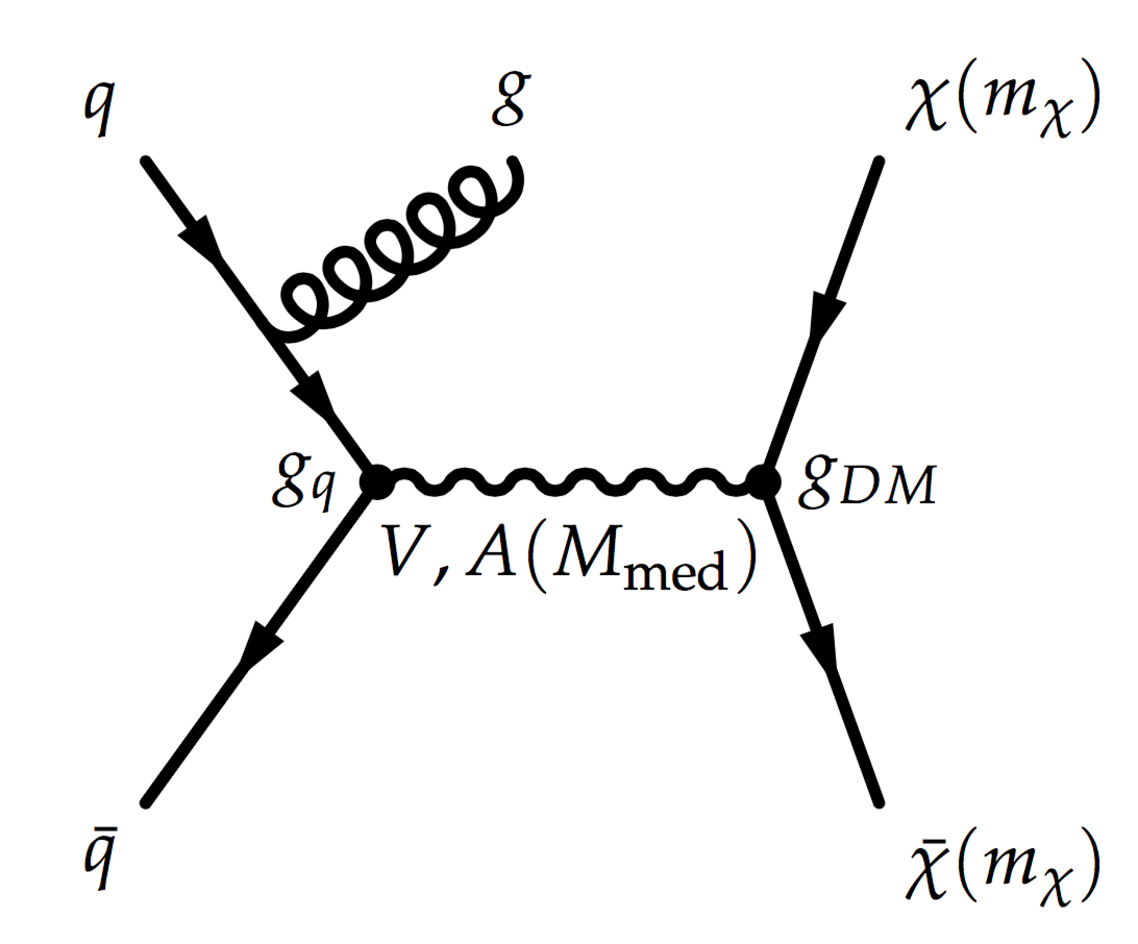
\includegraphics[width=0.5\textwidth]{figures/DMplots/feynman_light_jet.pdf}}
  \caption{Representative Feynman diagram showing the pair production of Dark Matter particles in association with a parton from the initial state via a vector or axial-vector mediator. The cross section and kinematics depend upon the mediator and Dark Matter masses, and the mediator couplings to Dark Matter and quarks respectively: ($m_{\Phi} ,\ m_\textrm{DM} ,\, g_{\textrm DM} ,\, g_{\textrm SM})$. \cite{Abercrombie:2015wmb}}
  \label{fig:feynman}
\end{figure}

$M_{\Phi}$ grid points are chosen, roughly equidistant in a logarithmic scale: 10,~20, 50, 100, 200, 300, 500, 1000 and 2000 GeV. In the thresh-
old regime $M_{\Phi} = 2 \times m_{\Chi}$, the $ m_{\Chi}$ grid points are taken at approximately $M_{\Phi}/2$. Points on the on-shell diagonal are always chosen to be
5 GeV away from the threshold, to avoid numerical instabilities in the event generation. 


\begin{table}[h!]
\centering
\begin{tabular}{l|llllllllll}\hline
mDM  & \multicolumn{10}{c}{mPhi}                                   \\ \hline
1    & 10 & 20 & 50 & 100 & 200 & 300 & 500 & 1000 & 2000 & 100000 \\
10   & 10 & 15 & 50 & 100 &     &     &     &      &      & 100000 \\
50   & 10 &    & 50 & 95  & 200 & 300 &     &      &      & 100000 \\
150  & 10 &    &    &     & 200 & 295 & 500 & 1000 &      & 100000 \\
500  & 10 &    &    &     &     &     & 500 & 995  &      & 100000 \\
1000 & 10 &    &    &     &     &     &     & 1000 & 1995 & 100000\\ \hline
\end{tabular}
\caption{Dark matter and mediator mass grid analysed. The parameter space follows the DM Forum recommendations~\cite{Abercrombie:2015wmb}}
\label{tab:DMgrid}
\end{table}

\subsection{Light Jet Models}


We consider four simplified models resulting in final states dominated by light quarks ($u,~d,~c,~s$) production. These models probe the axial-vector (A), vector (V), scalar (S) and pseudo-scalar (P) coupling of the mediator between dark matter and standard model particles. Currently the couplings constants $g_\textrm{DM}$ and $g_\textrm{SM}$ are assumed to be one. This document will be updated to reflect a recent recommendation of $g_\textrm{SM}=0.25$

Assuming 3 fb$^{-1}$ of data we list the expected efficiency and signal yield - divided into nominal and asymmetric selection - in Tables~\ref{tab:dm_A_g1_3fb}-\ref{tab:dm_P_g1_3fb}.

\begin{table}[h!]
\centering
\begin{tabular}{lllllll}
\hline
$m_\textrm{DM}$ & $m_\Phi$  & $\sigma$ [pb] & Sum Evts       & Evts Sym. Bin & Evts Asym. Bin & Eff  [\%]   \\\hline
1000 & 10000 & 3.68E-06 & 0        & 0        & 0        & 4.72 \\
1000 & 10    & 4.75E-04 & 0.06     & 0.03     & 0.03     & 3.86 \\
10 & 10000   & 1.21E-04 & 0.01     & 0        & 0        & 1.74 \\
10 & 10      & 1.26E+04 & 3304.45  & 1585.57  & 1718.88  & 0.01 \\
10 & 50      & 2.07E+05 & 51941.13 & 25290.54 & 26650.59 & 0.01 \\
150 & 1000   & 7.87E+00 & 768.58   & 353.3    & 415.28   & 3.25 \\
150 & 200    & 3.89E+00 & 125.17   & 59.45    & 65.72    & 1.07 \\
150 & 500    & 9.66E+01 & 3815.83  & 1816.58  & 1999.26  & 1.32 \\
1 & 1000     & 7.94E+00 & 826.75   & 389.3    & 437.45   & 3.47 \\
1 & 10       & 1.29E+07 & 22735.2  & 0        & 22735.2  & 0    \\
1 & 200      & 3.33E+03 & 30463.26 & 13629.37 & 16833.89 & 0.31 \\
1 & 300      & 5.97E+02 & 17418.02 & 8353.18  & 9064.84  & 0.97 \\
1 & 50       & 2.36E+05 & 56125.43 & 22631.23 & 33494.2  & 0.01 \\
500 & 10     & 1.50E-02 & 1.82     & 0.89     & 0.93     & 4.05 \\
500 & 500    & 3.27E-02 & 2.26     & 1.09     & 1.17     & 2.3  \\
50 & 10000   & 7.30E-05 & 0.01     & 0        & 0        & 2.89 \\
50 & 200     & 2.29E+03 & 25683.08 & 12110.16 & 13572.92 & 0.37 \\
50 & 50      & 1.15E+02 & 901.87   & 403.48   & 498.39   & 0.26\\
%100   &  400  & 6.89E+01 & 4685.76 & 2271.72 & 2414.04 & 2.27 \\
%10   &  1100  & 3.98E+00 & 192.57  & 91.15   & 101.42  & 1.61 \\
%10   &  800   & 1.25E+01 & 811.34  & 399.56  & 411.78  & 2.17 \\
%150   &  400  & 3.26E+01 & 1319.08 & 616.48  & 702.6   & 1.35 \\
%200   &  1100 & 2.46E+00 & 243.48  & 113.89  & 129.59  & 3.3  \\
%200   &  800  & 6.10E+00 & 544.81  & 252.92  & 291.89  & 2.98 \\
%250   &  400  & 3.07E+00 & 168.19  & 78.77   & 89.42   & 1.82 \\
%300   &  1100 & 1.57E+00 & 93.84   & 45.12   & 48.71   & 1.99 \\
%300   &  800  & 2.72E+00 & 207.65  & 100.6   & 107.05  & 2.55 \\
%350   &  400  & 6.01E-01 & 41.03   & 19.01   & 22.02   & 2.28 \\
%400   &  1100 & 8.33E-01 & 86.83   & 43.47   & 43.36   & 3.47 \\
%400   &  800  & 8.08E-01 & 97.91   & 46.89   & 51.02   & 4.04 \\
%450   &  400  & 1.86E-01 & 21.81   & 10.97   & 10.84   & 3.91 \\
%500   &  1100 & 3.41E-01 & 49.13   & 22.9    & 26.23   & 4.8  \\
%500   &  800  & 2.04E-01 & 17.94   & 8.44    & 9.5     & 2.93 \\
%50   &  400   & 1.06E+02 & 2660.98 & 1194.5  & 1466.48 & 0.84\\
\hline
\hline
\end{tabular}
\caption{Selected axial-vector samples. Given are production cross section, event yields for 3 fb$^{-1 }$ for the various selections and the overall selection efficiency for $g_\textrm{DM}=g_\textrm{SM}=1$}
\label{tab:dm_A_g1_3fb}
\end{table}


\begin{table}[h!]
\centering
\begin{tabular}{lllllll}
\hline
$m_\textrm{DM}$ & $m_\Phi$             & $\sigma$ [pb] & Sum Evts       & Evts Sym. Bin & Evts Asym. Bin & Eff  [\%]   \\\hline
1000 & 10000 & 1.20E-05 & 0        & 0        & 0        & 3.72 \\
1000 & 10    & 2.21E-03 & 0.23     & 0.12     & 0.11     & 3.44 \\
10 & 10000   & 6.72E-05 & 0.01     & 0        & 0        & 2.87 \\
10 & 10      & 3.44E+04 & 7286.95  & 4311.57  & 2975.38  & 0.01 \\
10 & 50      & 2.59E+05 & 74205.37 & 42898.33 & 31307.03 & 0.01 \\
150 & 1000   & 1.42E+01 & 813.7    & 402.16   & 411.53   & 1.91 \\
150 & 200    & 7.47E+00 & 335.71   & 156.75   & 178.96   & 1.5  \\
150 & 500    & 1.62E+02 & 5270.1   & 2602.18  & 2667.92  & 1.08 \\
1 & 1000     & 1.21E+01 & 806.66   & 386.29   & 420.36   & 2.21 \\
1 & 10       & 1.37E+07 & 44481.9  & 14432.4  & 30049.5  & 0    \\
1 & 200      & 3.15E+03 & 33252.25 & 13794.08 & 19458.17 & 0.35 \\
1 & 300      & 9.12E+02 & 17093.79 & 8309.57  & 8784.22  & 0.62 \\
1 & 50       & 2.55E+05 & 66536.46 & 33797.58 & 32738.88 & 0.01 \\
500 & 10     & 4.55E-02 & 5.48     & 2.71     & 2.77     & 4.01 \\
500 & 500    & 7.72E-02 & 7.71     & 3.79     & 3.92     & 3.33 \\
50 & 10000   & 7.42E-05 & 0.01     & 0        & 0        & 2.67 \\
50 & 200     & 4.30E+03 & 31005.5  & 13850.65 & 17154.85 & 0.24 \\
50 & 50      & 3.62E+02 & 1803.26  & 869.94   & 933.32   & 0.17 \\
%100   &  400  & 9.49E+01 & 3038.09 & 1445.03 & 1593.07 & 1.07 \\
%10   &  1100  & 3.89E+00 & 360.59  & 177.59  & 182.99  & 3.09 \\
%10   &  800   & 1.19E+01 & 692.38  & 317.41  & 374.97  & 1.94 \\
%150   &  400  & 6.98E+01 & 1943.39 & 923.21  & 1020.18 & 0.93 \\
%200   &  1100 & 3.28E+00 & 244.74  & 116.17  & 128.58  & 2.49 \\
%200   &  800  & 9.37E+00 & 745.95  & 346.92  & 399.03  & 2.65 \\
%250   &  400  & 1.08E+01 & 902.86  & 447.89  & 454.97  & 2.79 \\
%300   &  1100 & 2.73E+00 & 341.49  & 174.71  & 166.79  & 4.17 \\
%300   &  800  & 6.50E+00 & 392.12  & 184.01  & 208.11  & 2.01 \\
%350   &  400  & 1.99E+00 & 100.42  & 47.38   & 53.05   & 1.68 \\
%400   &  1100 & 2.02E+00 & 107.53  & 52.22   & 55.31   & 1.77 \\
%400   &  800  & 3.02E+00 & 242.18  & 117.44  & 124.74  & 2.67 \\
%450   &  400  & 6.24E-01 & 45.69   & 21.84   & 23.85   & 2.44 \\
%500   &  1100 & 1.18E+00 & 79.23   & 38.63   & 40.6    & 2.24 \\
%500   &  800  & 8.22E-01 & 70.33   & 33.94   & 36.39   & 2.85 \\
%50   &  400   & 1.08E+02 & 3248.04 & 1511.08 & 1736.96 & 1.00 \\
\hline
\end{tabular}
\caption{Selected vector samples. Given are production cross section, event yields for 3 fb$^{-1 }$ for the various selections and the overall selection efficiency for $g_\textrm{DM}=g_\textrm{SM}=1$}
\label{tab:dm_V_g1_3fb}
\end{table}




\clearpage
\subsubsection{Scalar and Pseudoscalar Models} \label{sec:dm_pscalar}

\begin{table}[h!]
\centering
\begin{tabular}{lllllll}
\hline
$m_\textrm{DM}$ & $m_\Phi$ & $\sigma$ [pb] & Sum Evts       & Evts Sym. Bin & Evts Asym. Bin & Eff  [\%]   \\\hline
1000  &  10000 & 1.74E-09 & 0      & 0      & 0      & 8.18 \\
1000  &  10    & 2.86E-07 & 0      & 0      & 0      & 7.55 \\
10  &  10000   & 4.53E-07 & 0      & 0      & 0      & 3.29 \\
10  &  10      & 1.23E+00 & 24.11  & 9.85   & 14.26  & 0.65 \\
10  &  50      & 3.45E+01 & 409.39 & 155.46 & 253.92 & 0.39 \\
150  &  1000   & 3.53E-02 & 4.67   & 2.29   & 2.38   & 4.41 \\
150  &  200    & 3.09E-02 & 2.23   & 0.95   & 1.28   & 2.4  \\
150  &  500    & 1.03E+00 & 78.62  & 34.64  & 43.98  & 2.55 \\
1  &  1000     & 4.09E-02 & 5.38   & 2.65   & 2.73   & 4.38 \\
1  &  10       & 6.10E+01 & 439.55 & 219.77 & 219.77 & 0.24 \\
1  &  200      & 6.79E+00 & 267.37 & 111.53 & 155.84 & 1.31 \\
1  &  300      & 4.18E+00 & 215.57 & 90.37  & 125.2  & 1.72 \\
1  &  50       & 3.44E+01 & 361.38 & 157.46 & 203.92 & 0.35 \\
500  &  10     & 4.95E-05 & 0.01   & 0      & 0      & 5.64 \\
500  &  500    & 6.79E-05 & 0.01   & 0.01   & 0.01   & 5.82 \\
50  &  10000   & 4.22E-07 & 0      & 0      & 0      & 3.3  \\
50  &  200     & 6.81E+00 & 282.31 & 112.82 & 169.49 & 1.38 \\
50  &  50      & 1.76E-01 & 8.4    & 3.53   & 4.87   & 1.59 \\
%100   &  350 & 2.31E+00 & 126.62 & 53.47  & 73.15  & 1.82 \\
%10   &  225  & 5.71E+00 & 266.19 & 95.96  & 170.22 & 1.55 \\
%10   &  50   & 2.66E+01 & 295.33 & 114.41 & 180.93 & 0.37 \\
%125   &  400 & 1.59E+00 & 89.97  & 39.81  & 50.16  & 1.88 \\
%150   &  400 & 9.79E-01 & 59.63  & 24.09  & 35.54  & 2.03 \\
%15   &  250  & 4.94E+00 & 239.01 & 106.17 & 132.84 & 1.61 \\
%15   &  75   & 1.84E+01 & 337.76 & 122.99 & 214.77 & 0.61 \\
%1   &  25    & 5.02E+01 & 430.66 & 186.79 & 243.87 & 0.29 \\
%200   &  275 & 1.23E-02 & 1.06   & 0.49   & 0.57   & 2.86 \\
%20   &  150  & 9.07E+00 & 275.78 & 116.12 & 159.66 & 1.01 \\
%20   &  400  & 3.30E+00 & 203.51 & 90.19  & 113.32 & 2.05 \\
%35   &  225  & 4.96E+00 & 218.64 & 94.7   & 123.95 & 1.47 \\
%35   &  50   & 3.44E-01 & 11.95  & 5.37   & 6.58   & 1.16 \\
%50   &  275  & 3.66E+00 & 192.7  & 81.17  & 111.52 & 1.76 \\
%5   &  10    & 3.81E+00 & 46.88  & 19.82  & 27.06  & 0.41 \\
%5   &  300   & 4.18E+00 & 221.37 & 94.39  & 126.97 & 1.77 \\
%75   &  150  & 3.18E-01 & 13.47  & 5.21   & 8.26   & 1.41 \\
%75   &  450  & 1.82E+00 & 120.5  & 56.16  & 64.34  & 2.21\\
\hline
\end{tabular}
\caption{Selected scalar samples. Given are production cross section, event yields for 3 fb$^{-1 }$ for the various selections and the overall selection efficiency for $g_\textrm{DM}=g_\textrm{SM}=1$}
\label{tab:dm_S_g1_3fb}
\end{table}


\begin{table}[h!]
\centering
\begin{tabular}{lllllll}
\hline
$m_\textrm{DM}$ & $m_\Phi$             & $\sigma$ [pb] & Sum Evts       & Evts Sym. Bin & Evts Asym. Bin & Eff  [\%]   \\\hline
1000  & 10000 & 5.26E-09 & 0       & 0      & 0       & 7.87 \\
1000  & 10    & 1.27E-06 & 0       & 0      & 0       & 7.56 \\
10  & 10000   & 8.67E-07 & 0       & 0      & 0       & 2.9  \\
10  & 10      & 3.87E+00 & 69.93   & 29.3   & 40.62   & 0.6  \\
10  & 50      & 7.80E+01 & 1310.12 & 187.16 & 1122.96 & 0.56 \\
150  & 1000   & 4.95E-02 & 6.61    & 3.59   & 3.01    & 4.45 \\
150  & 200    & 2.00E-01 & 12.34   & 5.38   & 6.95    & 2.05 \\
150  & 500    & 1.80E+00 & 144.8   & 67.06  & 77.74   & 2.68 \\
1  & 1000     & 5.42E-02 & 6.81    & 3.42   & 3.39    & 4.18 \\
1  & 10       & 1.37E+02 & 1133.59 & 474.05 & 659.54  & 0.27 \\
1  & 200      & 1.67E+01 & 695.99  & 279.17 & 416.82  & 1.39 \\
1  & 300      & 1.27E+01 & 799.84  & 380.88 & 418.97  & 2.1  \\
1  & 50       & 7.79E+01 & 935.04  & 395.6  & 539.45  & 0.4  \\
500  & 10     & 1.94E-04 & 0.03    & 0.02   & 0.01    & 5.43 \\
500  & 500    & 2.85E-04 & 0.05    & 0.03   & 0.02    & 5.6  \\
50  & 10000   & 8.36E-07 & 0       & 0      & 0       & 2.65 \\
50  & 200     & 1.67E+01 & 681.41  & 220.46 & 460.95  & 1.36 \\
50  & 50      & 7.06E-01 & 22.58   & 8.47   & 14.11   & 1.07\\
%100   &  350 & 1.25E+01 & 632.71  & 265.81  & 366.9   & 1.69 \\
%10   &  200  & 1.66E+01 & 668.92  & 282.88  & 386.04  & 1.34 \\
%10   &  500  & 2.10E+00 & 165.24  & 70.13   & 95.12   & 2.62 \\
%125   &  350 & 1.06E+01 & 574.48  & 230.85  & 343.62  & 1.8  \\
%150   &  350 & 7.83E+00 & 389.76  & 154.97  & 234.8   & 1.66 \\
%15   &  250  & 1.33E+01 & 631.37  & 262.63  & 368.74  & 1.59 \\
%15   &  75   & 4.97E+01 & 809.62  & 302.99  & 506.63  & 0.54 \\
%1   &  25    & 1.14E+02 & 1013.45 & 375.77  & 637.68  & 0.3  \\
%200   &  275 & 7.09E-02 & 5.52    & 2.42    & 3.1     & 2.6  \\
%20   &  150  & 2.30E+01 & 709.86  & 281.18  & 428.68  & 1.03 \\
%20   &  400  & 6.73E+00 & 389.39  & 158.04  & 231.34  & 1.93 \\
%35   &  225  & 1.40E+01 & 601.6   & 249.85  & 351.75  & 1.44 \\
%35   &  50   & 1.41E+00 & 38.92   & 14.67   & 24.26   & 0.92 \\
%50   &  275  & 1.18E+01 & 564.9   & 220.54  & 344.37  & 1.6  \\
%5   &  10    & 8.66E+02 & 5888.89 & 3117.65 & 2771.24 & 0.23 \\
%5   &  300   & 1.27E+01 & 657.28  & 263.93  & 393.35  & 1.73 \\
%75   &  150  & 9.49E+01 & 3199.78 & 1300.8  & 1898.98 & 1.12 \\
%75   &  450  & 3.39E+00 & 237.3   & 106.45  & 130.86  & 2.33 \\
\hline
\end{tabular}
\caption{Selected pseudo-scalar samples. Given are production cross section, event yields for 3 fb$^{-1 }$ for the various selections and the overall selection efficiency for $g_\textrm{DM}=g_\textrm{SM}=1$}
\label{tab:dm_P_g1_3fb}
\end{table}



\subsubsection{Projected sensitivities}

The 'R' value is the relative signal strength required to exclude a given model in the selection probed. Smaller values indicate better sensitivities and $R=1$ denotes the value at which a particular point is excluded. Expected R values for simplified dark matter models using scalar and pseudo-scalar couplings are calculated for 3 fb$^{-1 }$ and 10 fb$^{-1 }$. Table~\ref{tab:dm_A_R_values} lists these
values for the DM and mediator masses $m_\textrm{DM}$, $m_\Phi$ recommended by the DM forum for the axial operator. The corresponding results for the vector couplings are given in Table~\ref{tab:dm_V_R_values}. Table~\ref{tab:dm_S_R_values} lists the scalar and Table~\ref{tab:dm_P_R_values} the pseudo-scalar models.



\begin{table}[h!]
\centering
\begin{tabular}{llll}
\hline                      
 $m_\textrm{DM}$ & $m_\Phi$  & R 3 fb$^{-1}$ & R 10 fb$^{-1}$ \\ \hline

1  &       10  &      0.01  &    0.00 \\\hline
1  &       20  &      0.00  &    0.00 \\\hline
1  &       50  &      0.00  &    0.00 \\\hline
1  &       100  &     0.00  &    0.00 \\\hline
1  &       200  &     0.01  &    0.01 \\\hline
1  &       300  &     0.02  &    0.01 \\\hline
1  &       500  &     0.06  &    0.03 \\\hline
1  &       1000  &    0.39  &    0.21 \\\hline
1  &       2000  &    4.39  &    2.38 \\\hline
10  &      10  &      0.05  &    0.03 \\\hline
10  &      15  &      0.03  &    0.02 \\\hline
10  &      50  &      0.00  &    0.00 \\\hline
10  &      100  &     0.00  &    0.00 \\\hline
10  &      10000  &   201.50  &  668.50 \\\hline
50  &      10  &      0.39  &    0.20 \\\hline
50  &      50  &      0.38  &    0.21 \\\hline
50  &      95  &      0.18  &    0.10 \\\hline
50  &      200  &     0.01  &    0.01 \\\hline
50  &      300  &     0.02  &    0.01 \\\hline
50  &      10000  &   97.75  &   324.50 \\\hline
150  &     10  &      3.58  &    1.91 \\\hline
150  &     200  &     2.70  &    1.44 \\\hline
150  &     295  &     0.96  &    0.52 \\\hline
150  &     500  &     0.09  &    0.05 \\\hline
150  &     1000  &    0.40  &    0.23 \\\hline
150  &     10000  &   -     &  4000.00   \\ \hline
500  &     10  &      148.75  &  81.25 \\\hline
500  &     500  &     126.25  &  68.25 \\\hline
500  &     995  &     21.06  &   11.28 \\\hline
500  &     2000  &    6.11  &    3.39 \\\hline
1000 &   1000    &-         & 2017.75 \\ \hline
1000  &    1995  &    323.00  &  169.81 \\\hline
%1       & 10      & 0.81    & 0.56 \\ \hline
%1       & 20      & 0.16    & 0.1 \\ \hline
%1       & 50      & 0.06    & 0.04 \\ \hline
%1       & 100     & 0.06    & 0.03 \\ \hline
%1       & 200     & 0.07    & 0.04 \\ \hline
%1       & 300     & 0.07    & 0.04 \\ \hline
%1       & 500     & 0.26    & 0.14 \\ \hline
%1       & 1000    & 0.91    & 0.49 \\ \hline
%1       & 2000    & 13.06   & 7.09 \\ \hline
%10      & 10      & 1.28    & 0.72 \\ \hline
%10      & 15      & 1.07    & 0.6 \\ \hline
%10      & 50      & 0.03    & 0.01 \\ \hline
%10      & 100     & 0.05    & 0.03 \\ \hline
%10      & 10000   & 205.5   & 672.5 \\ \hline
%50      & 10      & 3.14    & 1.57 \\ \hline
%50      & 50      & 2.8     & 1.55 \\ \hline
%50      & 95      & 1.18    & 0.63 \\ \hline
%50      & 200     & 0.08    & 0.04 \\ \hline
%50      & 300     & 0.1     & 0.06 \\ \hline
%50      & 10000   & 98.75   & 326.5 \\ \hline
%150     & 10      & 10.09   & 5.39 \\ \hline
%150     & 200     & 12.56   & 6.72 \\ \hline
%150     & 295     & 3.95    & 2.12 \\ \hline
%150     & 500     & 0.37    & 0.2 \\ \hline
%150     & 1000    & 1.04    & 0.59 \\ \hline
%500     & 10      & 373.63  & 204.25 \\ \hline
%500     & 500     & 530.25  & 287 \\ \hline
%500     & 995     & 71.91   & 38.38 \\ \hline
%500     & 2000    & 13.19   & 7.34 \\ \hline
%1000    & 1995    & 391.5   & 402.63 \\ \hline
\end{tabular}
\caption{Projected R values for 3 fb$^{-1}$ and 10 fb$^{-1}$} for the axial-vector models.
\label{tab:dm_A_R_values}
\end{table}


\begin{table}[h!]
\centering
\begin{tabular}{llll}
\hline                      
 $m_\textrm{DM}$ & $m_\Phi$  & R 3 fb$^{-1}$ & R 10 fb$^{-1}$ \\ \hline


1  &       10  &      0.00  &    0.01 \\\hline
1  &       20  &      0.00  &    0.00 \\\hline
1  &       50  &      0.00  &    0.00 \\\hline
1  &       100  &     0.00  &    0.00 \\\hline
1  &       200  &     0.01  &    0.01 \\\hline
1  &       300  &     0.00  &    0.01 \\\hline
1  &       500  &     0.06  &    0.03 \\\hline
1  &       1000  &    0.36  &    0.20 \\\hline
1  &       2000  &    4.39  &    2.32 \\\hline
10  &      10  &      0.02  &    0.01 \\\hline
10  &      15  &      0.02  &    0.01 \\\hline
10  &      50  &      0.00  &    0.00 \\\hline
10  &      100  &     0.00  &    0.00 \\\hline
10  &    10000  &  4000.00 & - \\\hline
50  &      10  &      0.22  &    0.11 \\\hline
50  &      50  &      0.19  &    0.10 \\\hline
50  &      95  &      0.05  &    0.02 \\\hline
50  &      200  &     0.01  &    0.01 \\\hline
50  &      300  &     0.02  &    0.01 \\\hline
50  &    10000  &  4000.00  &   - \\ \hline
150  &     10  &      1.82  &    0.98 \\\hline
150  &     200  &     1.11  &    0.60 \\\hline
150  &     295  &     0.14  &    0.07 \\\hline
150  &     500  &     0.07  &    0.04 \\\hline
150  &     1000  &    0.30  &    0.16 \\\hline
500  &     10  &      52.81  &   28.63 \\\hline
500  &     500  &     37.91  &   21.44 \\\hline
500  &     995  &     1.87  &    1.04 \\\hline
500  &     2000  &    4.73  &    2.52 \\\hline
500  &     10000  &   4000.00  & - \\ \hline
1000  &    10  &       1166.25  & 559.94 \\\hline
1000  &    1000  &    788.88  & 406.00 \\\hline
1000  &    1995  &    22.19  & 12.09 \\\hline
1000  &    10000  &   616.5  &   2002.50 \\\hline
%1       & 10      & 0.10    & 0.04 \\ \hline
%1       & 20      & 0.09    & 0.05 \\ \hline
%1       & 50      & 0.06    & 0.03 \\ \hline
%1       & 100     & 0.05    & 0.03 \\ \hline
%1       & 200     & 0.07    & 0.04 \\ \hline
%1       & 300     & 0.11    & 0.06 \\ \hline
%1       & 500     & 0.30    & 0.17 \\ \hline
%1       & 1000    & 1.30    & 0.71 \\ \hline
%1       & 2000    & 5.61    & 2.98 \\ \hline
%10      & 10      & 0.66    & 0.39 \\ \hline
%10      & 15      & 0.70    & 0.35 \\ \hline
%10      & 50      & 0.04    & 0.02 \\ \hline
%10      & 100     & 0.03    & 0.02 \\ \hline
%50      & 10      & 1.99    & 1.01 \\ \hline
%50      & 50      & 1.74    & 0.97 \\ \hline
%50      & 95      & 0.48    & 0.25 \\ \hline
%50      & 200     & 0.09    & 0.05 \\ \hline
%50      & 300     & 0.13    & 0.07 \\ \hline
%150     & 10      & 6.81    & 3.67 \\ \hline
%150     & 200     & 3.20    & 1.72 \\ \hline
%150     & 295     & 0.60    & 0.33 \\ \hline
%150     & 500     & 0.32    & 0.18 \\ \hline
%150     & 1000    & 1.29    & 0.71 \\ \hline
%500     & 10      & 123.63  & 67.25 \\ \hline
%500     & 500     & 106.25  & 60.25 \\ \hline
%500     & 995     & 7.84    & 4.39 \\ \hline
%500     & 2000    & 11.28   & 6.02 \\ \hline
%1000    & 1995    & 62.63   & 34.13 \\ \hline
%1000    & 10000   & 669.50  & 1399.50 \\ \hline
\end{tabular}
\caption{Projected R values for 3 fb$^{-1}$ and 10 fb$^{-1}$} for the vector models.
\label{tab:dm_V_R_values}
\end{table}


Expected exclusion contours for the vector and axial-vector couplings at 95\% CL can be found in Figs.~\ref{fig:limits_V}-\ref{fig:limits_A}. The projection are performed for  3\fbinv and 10\fbinv of luminosity.

\begin{figure}[h!]
  \centering
  \subfigure{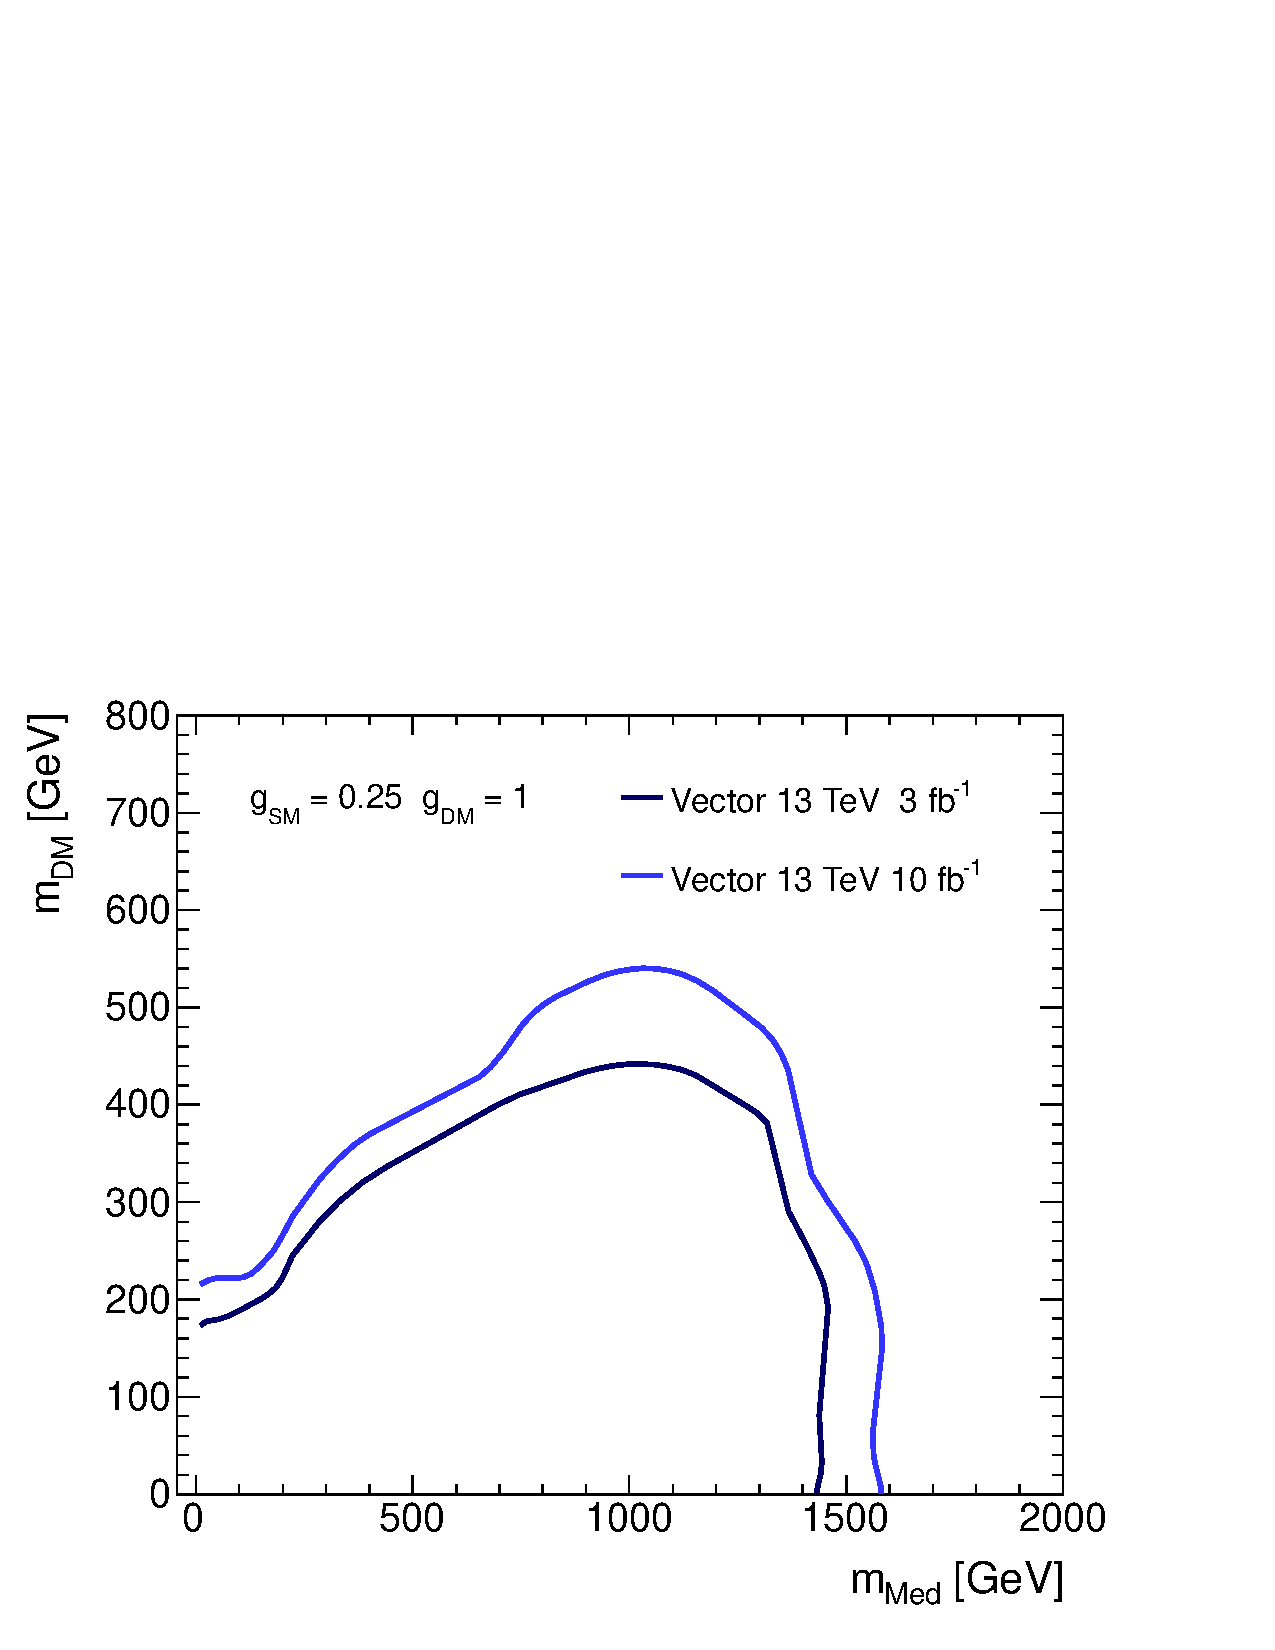
\includegraphics[width=0.5\textwidth]{figures/DMplots/justVlin.pdf}}
  \subfigure{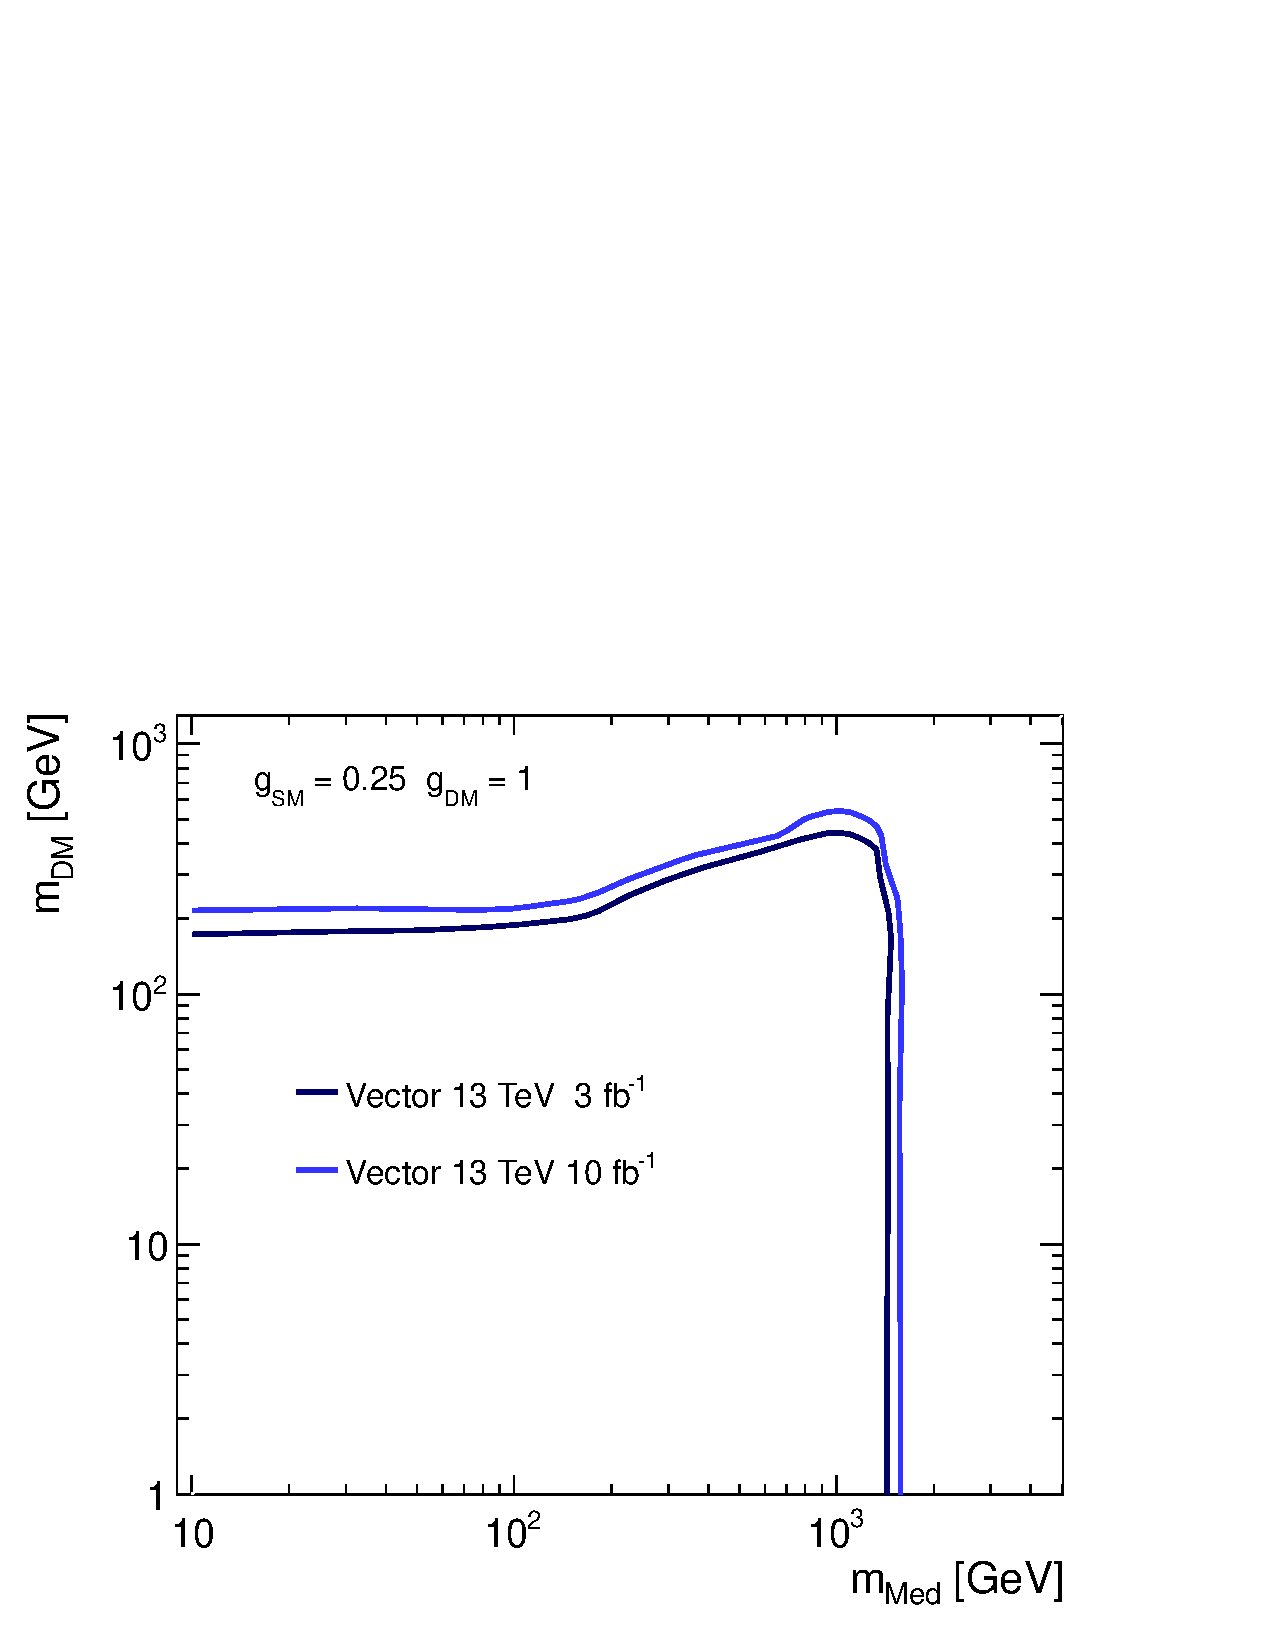
\includegraphics[width=0.5\textwidth]{figures/DMplots/justVlog.pdf}}
  \caption{\label{fig:limits_V} Expected exclusion contours at 95\% CL for 3\fbinv and 10\fbinv using vector couplings. }
\end{figure}


\begin{figure}[h!]
  \centering
  \subfigure{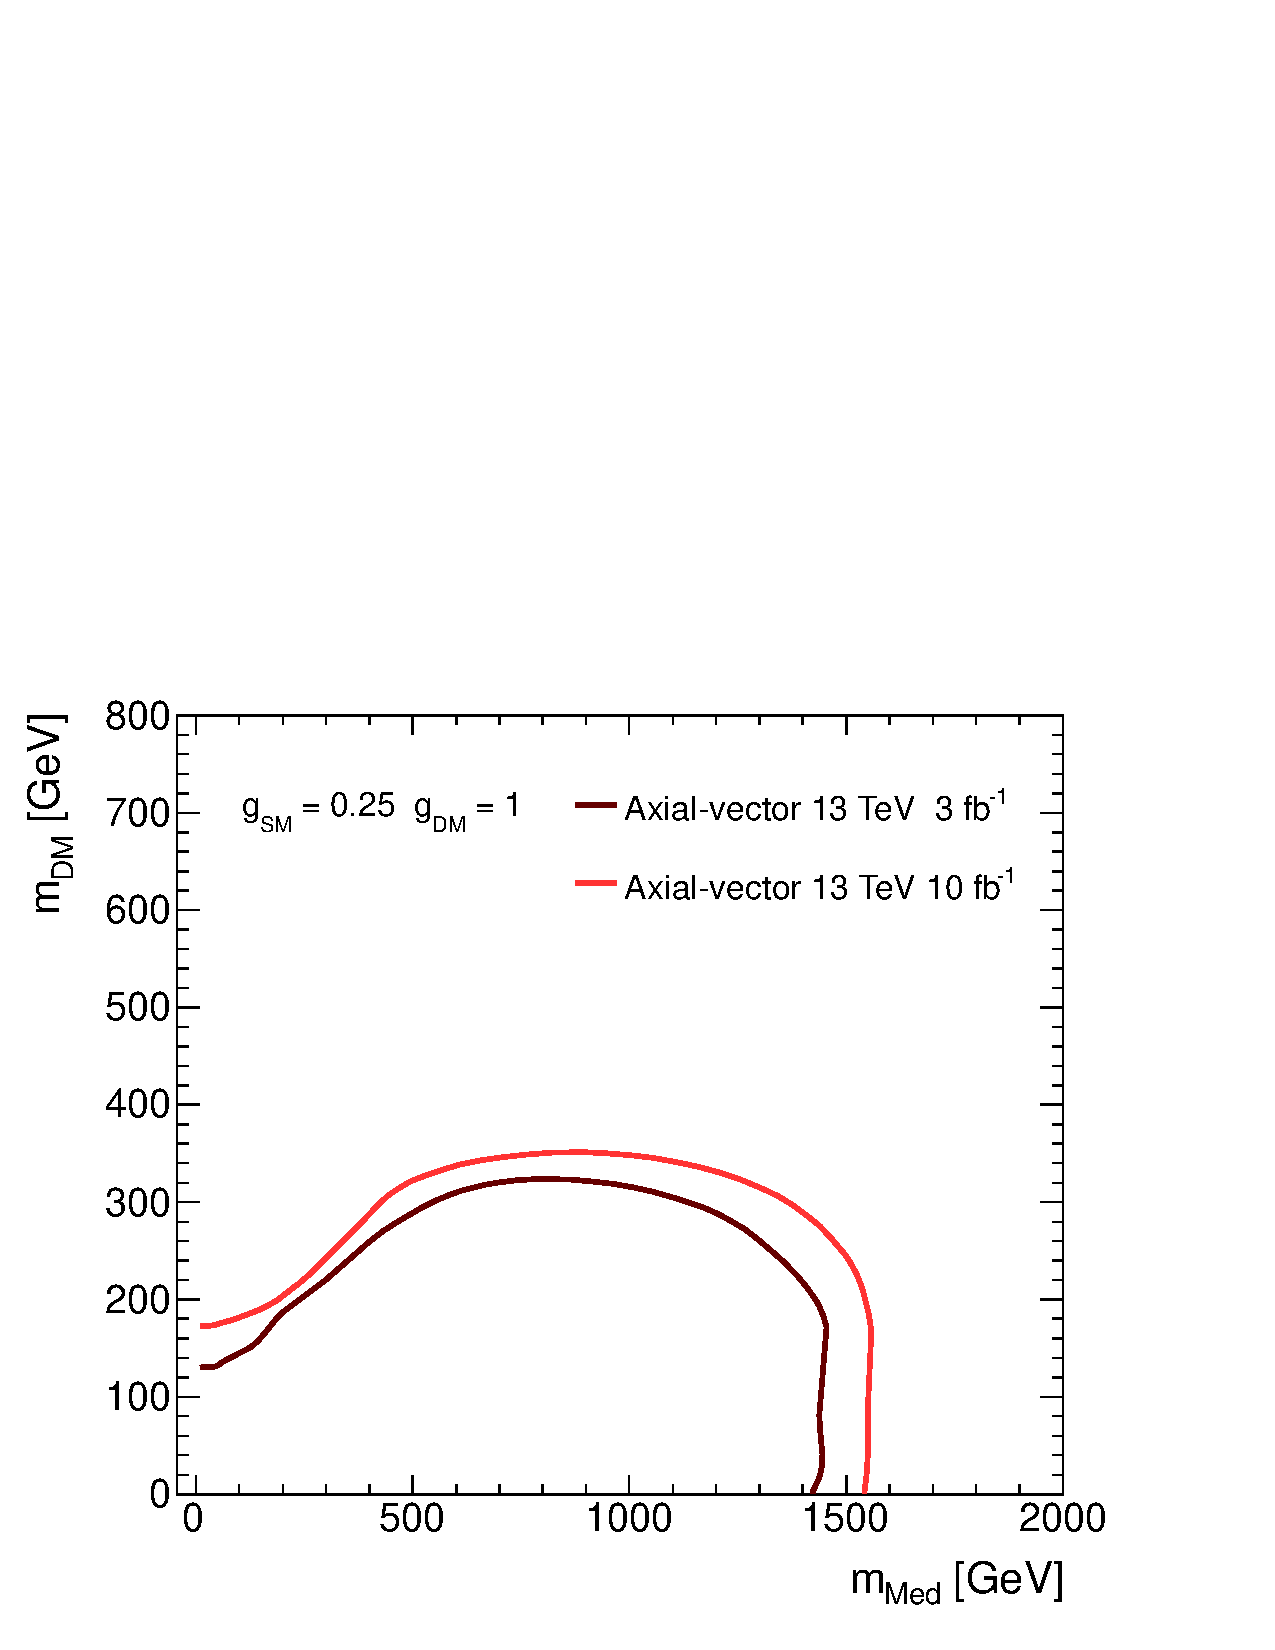
\includegraphics[width=0.5\textwidth]{figures/DMplots/justAlin.pdf}}
  \subfigure{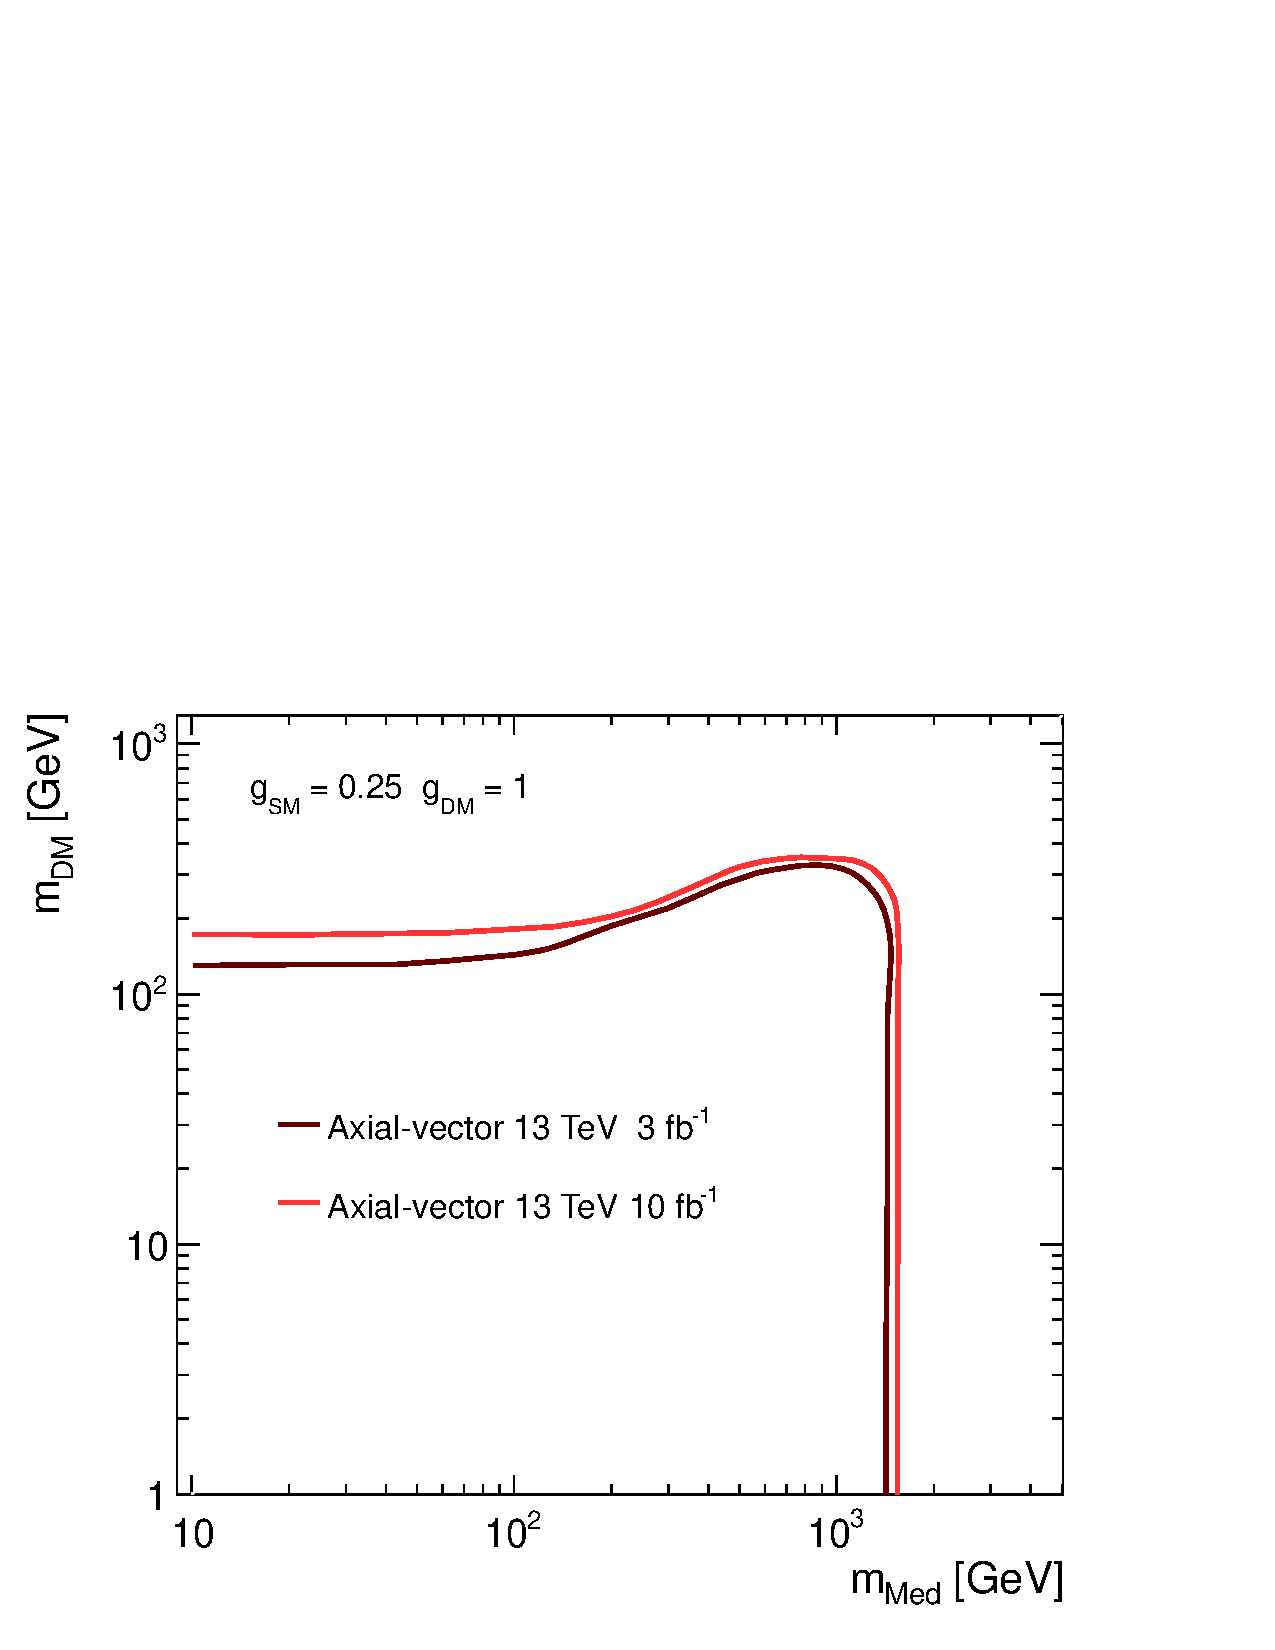
\includegraphics[width=0.5\textwidth]{figures/DMplots/justAlog.pdf}}
  \caption{\label{fig:limits_A} Expected exclusion contours at 95\% CL for 3\fbinv and 10\fbinv using axial-vector couplings. }
\end{figure}


\begin{table}[h!]
  \centering
  \begin{tabular}{llll}
    \hline                      
    $m_\textrm{DM}$ & $m_\Phi$  & R 3 fb$^{-1}$ & R 10 fb$^{-1}$ \\ \hlin
    1	& 10	& 0.54	& 0.30 \\ \hline
    1	& 20	& 0.61	& 0.32 \\ \hline
    1	& 50	& 0.60	& 0.33 \\ \hline
    1	& 100	& 0.72	& 0.39 \\ \hline
    1	& 200	& 1.26	& 0.69 \\ \hline
    1	& 300	& 1.79	& 1.00 \\ \hline
    1	& 500	& 3.55	& 1.98 \\ \hline
    1	& 1000	& 59.97	& 32.38 \\ \hline
    1	& 2000	& -    & 1679.75 \\ \hline
    10	& 10	& 11.91	& 6.34 \\ \hline 
    10	& 15	& 11.41	& 6.28 \\ \hline
    10	& 50	& 0.61	& 0.32 \\ \hline
    10	& 100	& 0.70	& 0.40 \\ \hline
    50	& 10	& 45.63	& 24.31 \\ \hline
    50	& 50	& 38.88	& 20.19 \\ \hline
    50	& 95	& 25.13	& 13.56 \\ \hline
    50	& 200	& 1.24	& 0.69 \\ \hline
    50	& 300	& 1.71	& 0.93 \\ \hline
    150	& 10	& 232.25& 128.25 \\ \hline
    150	& 200	& 158.25& 86.81 \\ \hline
    150	& 295	& 62.50	& 33.88 \\ \hline
    150	& 500	& 4.64	& 2.48 \\ \hline
    150	& 1000	& 68.81	& 36.63 \\ \hline
  \end{tabular}
  \caption{Projected R values for 3 fb$^{-1}$ and 10 fb$^{-1}$ for the scalar models. \label{tab:dm_S_R_values}}
\end{table}


\begin{table}[h!]
  \centering
  \begin{tabular}{llll}
    \hline                      
    $m_\textrm{DM}$ & $m_\Phi$  & R 3 fb$^{-1}$ & R 10 fb$^{-1}$ \\ \hline
    1       & 10      & 0.18    & 0.10 \\ \hline
    1       & 20      & 0.21    & 0.13 \\ \hline
    1       & 50      & 0.26    & 0.14 \\ \hline
    1       & 100     & 0.04    & 0.02 \\ \hline
    1       & 200     & 0.53    & 0.29 \\ \hline
    1       & 300     & 0.10    & 0.05 \\ \hline
    1       & 500     & 2.29    & 1.28 \\ \hline
    1       & 1000    & 44.38   & 23.31 \\ \hline
    1       & 2000    & 3003.50 & 1036.50 \\ \hline
    10      & 10      & 3.58    & 1.88 \\ \hline
    10      & 15      & 3.67    & 1.91 \\ \hline
    10      & 50      & 0.05    & 0.02 \\ \hline
    10      & 100     & 0.34    & 0.19 \\ \hline
    50      & 10      & 11.97   & 6.34 \\ \hline
    50      & 50      & 3.52    & 2.02 \\ \hline
    50      & 95      & 0.86    & 0.46 \\ \hline
    50      & 200     & 0.16    & 0.08 \\ \hline
    50      & 300     & 0.51    & 0.28 \\ \hline
    150     & 10      & 50.81   & 27.13 \\ \hline
    150     & 200     & 28.38   & 15.31 \\ \hline
    150     & 295     & 4.92    & 2.71 \\ \hline
    150     & 500     & 2.51    & 1.39 \\ \hline
    150     & 1000    & 39.38   & 20.91 \\ \hline
    500     & 995     & 308.25  & 170.81 \\ \hline
    500     & 2000    & -       & 1591.50 \\ \hline
    1000    & 10      & -       & 4000.00 \\ \hline
  \end{tabular}
  \caption{Projected R values for 3 fb$^{-1}$ and 10 fb$^{-1}$ for the pseudo-scalar models. \label{tab:dm_P_R_values}}
\end{table}



Expected exclusion contours for the vector and axial-vector couplings at 95\% CL can be found in Figs.~\ref{fig:limits_S}-\ref{fig:limits_P}. The projection are performed for 3\fbinv and 10\fbinv of luminosity.


\begin{figure}[h!]
  \centering
  \subfigure{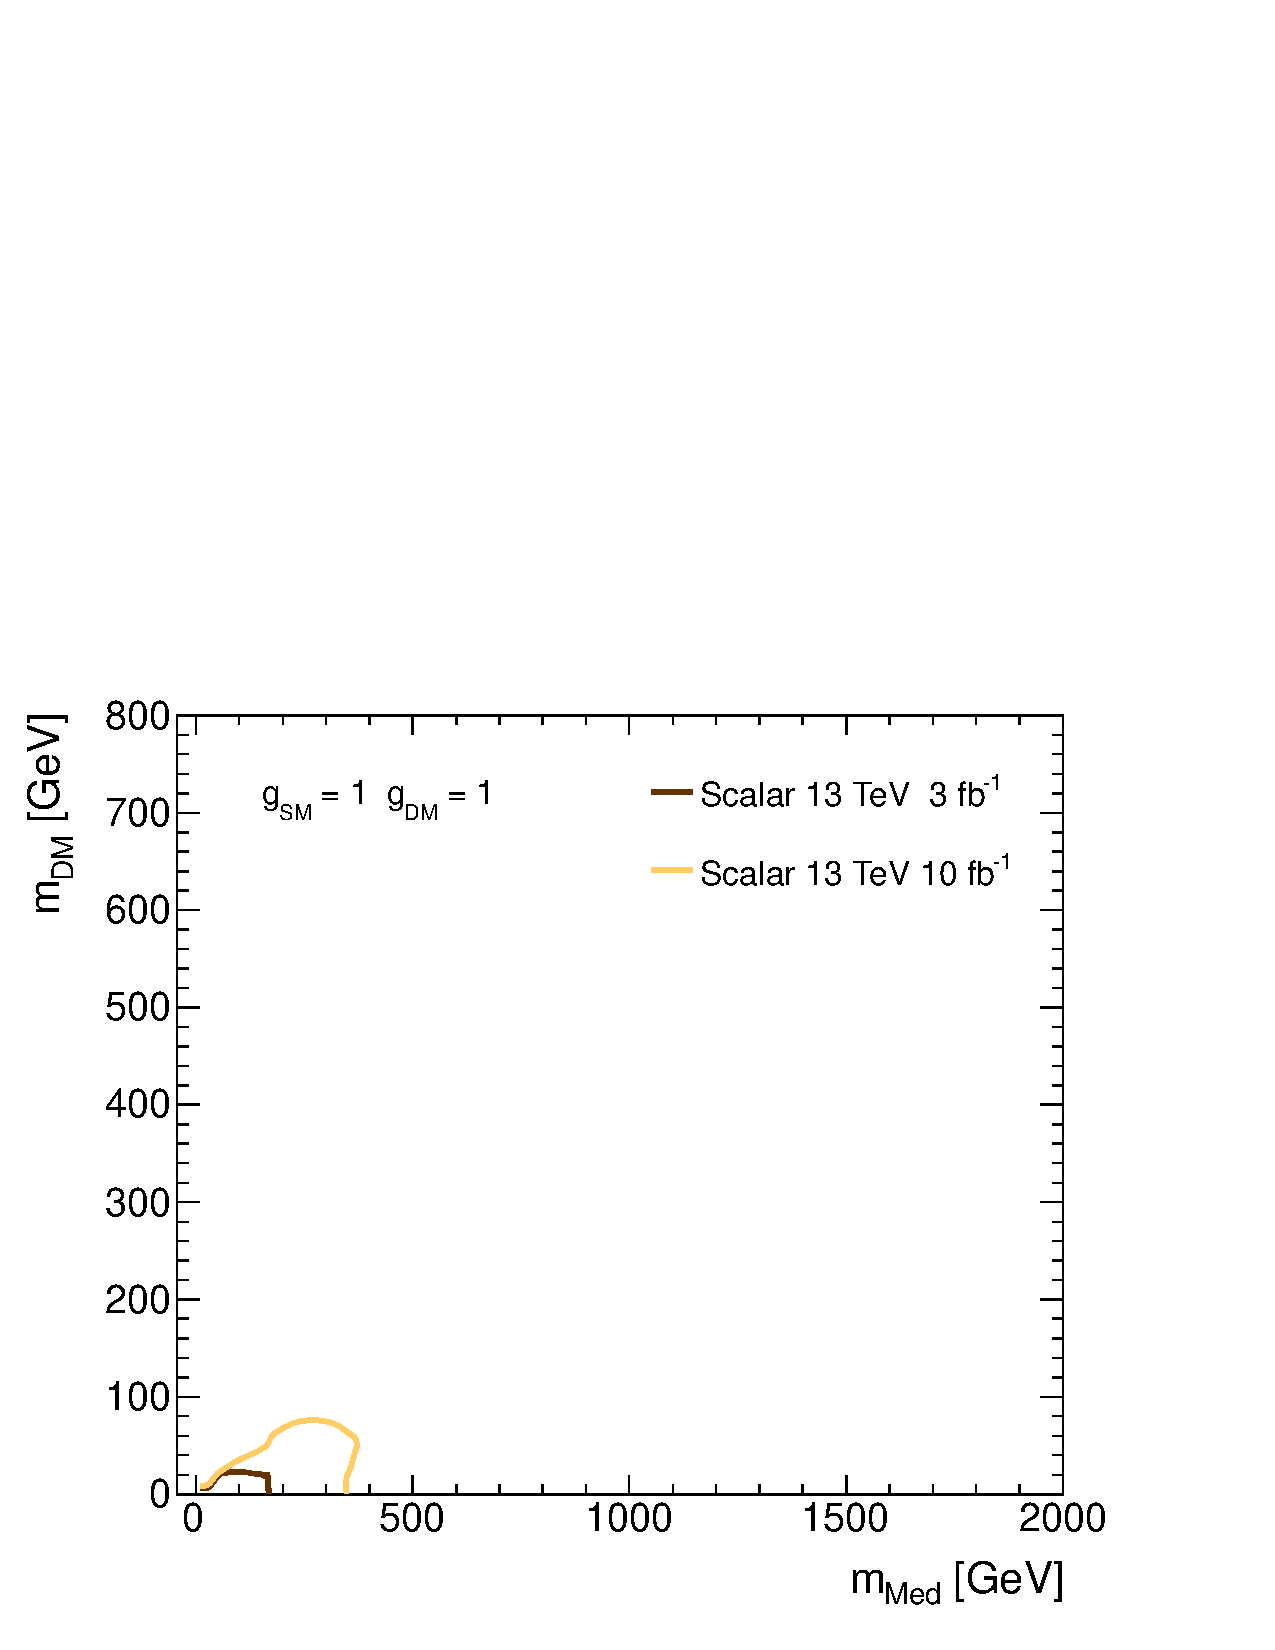
\includegraphics[width=0.5\textwidth]{figures/DMplots/justSlin.pdf}}
  \subfigure{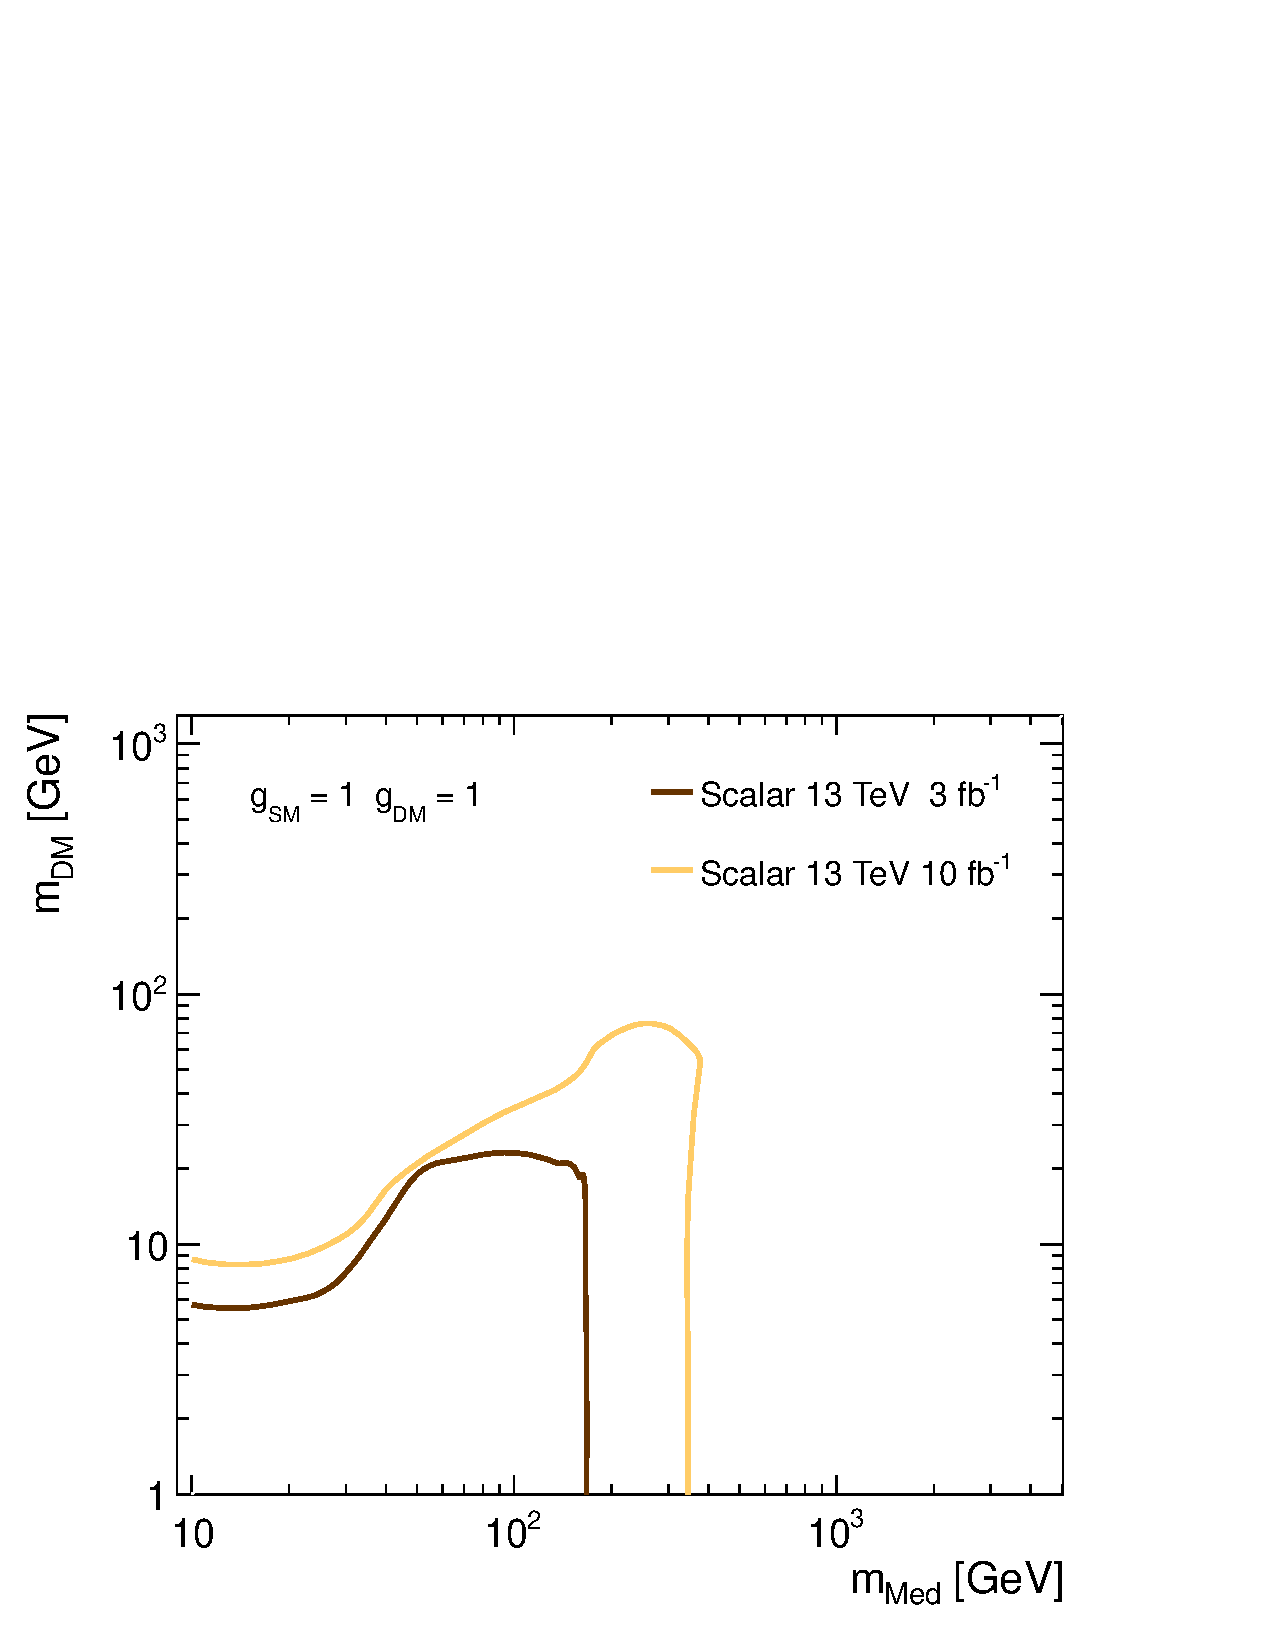
\includegraphics[width=0.5\textwidth]{figures/DMplots/justSlog.pdf}}
  \caption{\label{fig:limits_S} Expected exclusion contours at 95\% CL for 3\fbinv and 10\fbinv using scalar couplings. }
\end{figure}


\begin{figure}[h!]
  \centering
  \subfigure{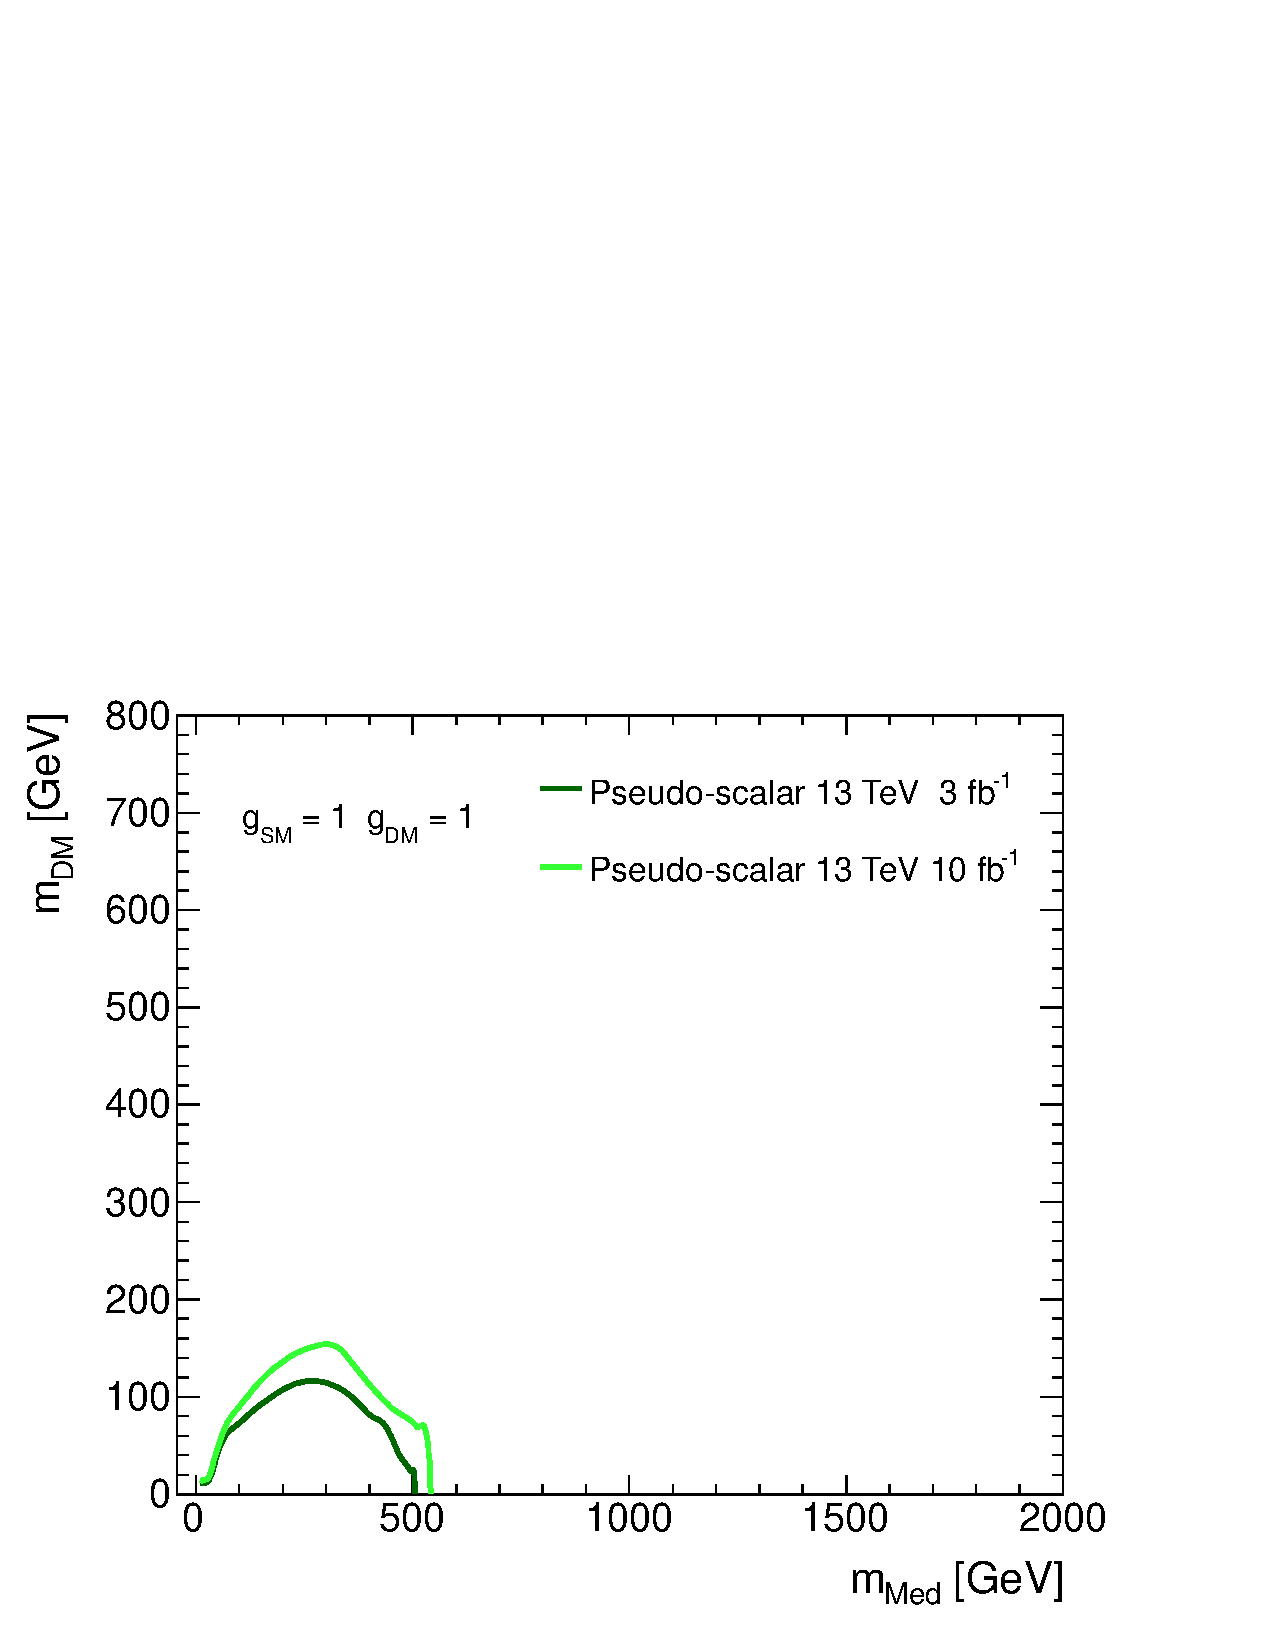
\includegraphics[width=0.5\textwidth]{figures/DMplots/justPlin.pdf}}
  \subfigure{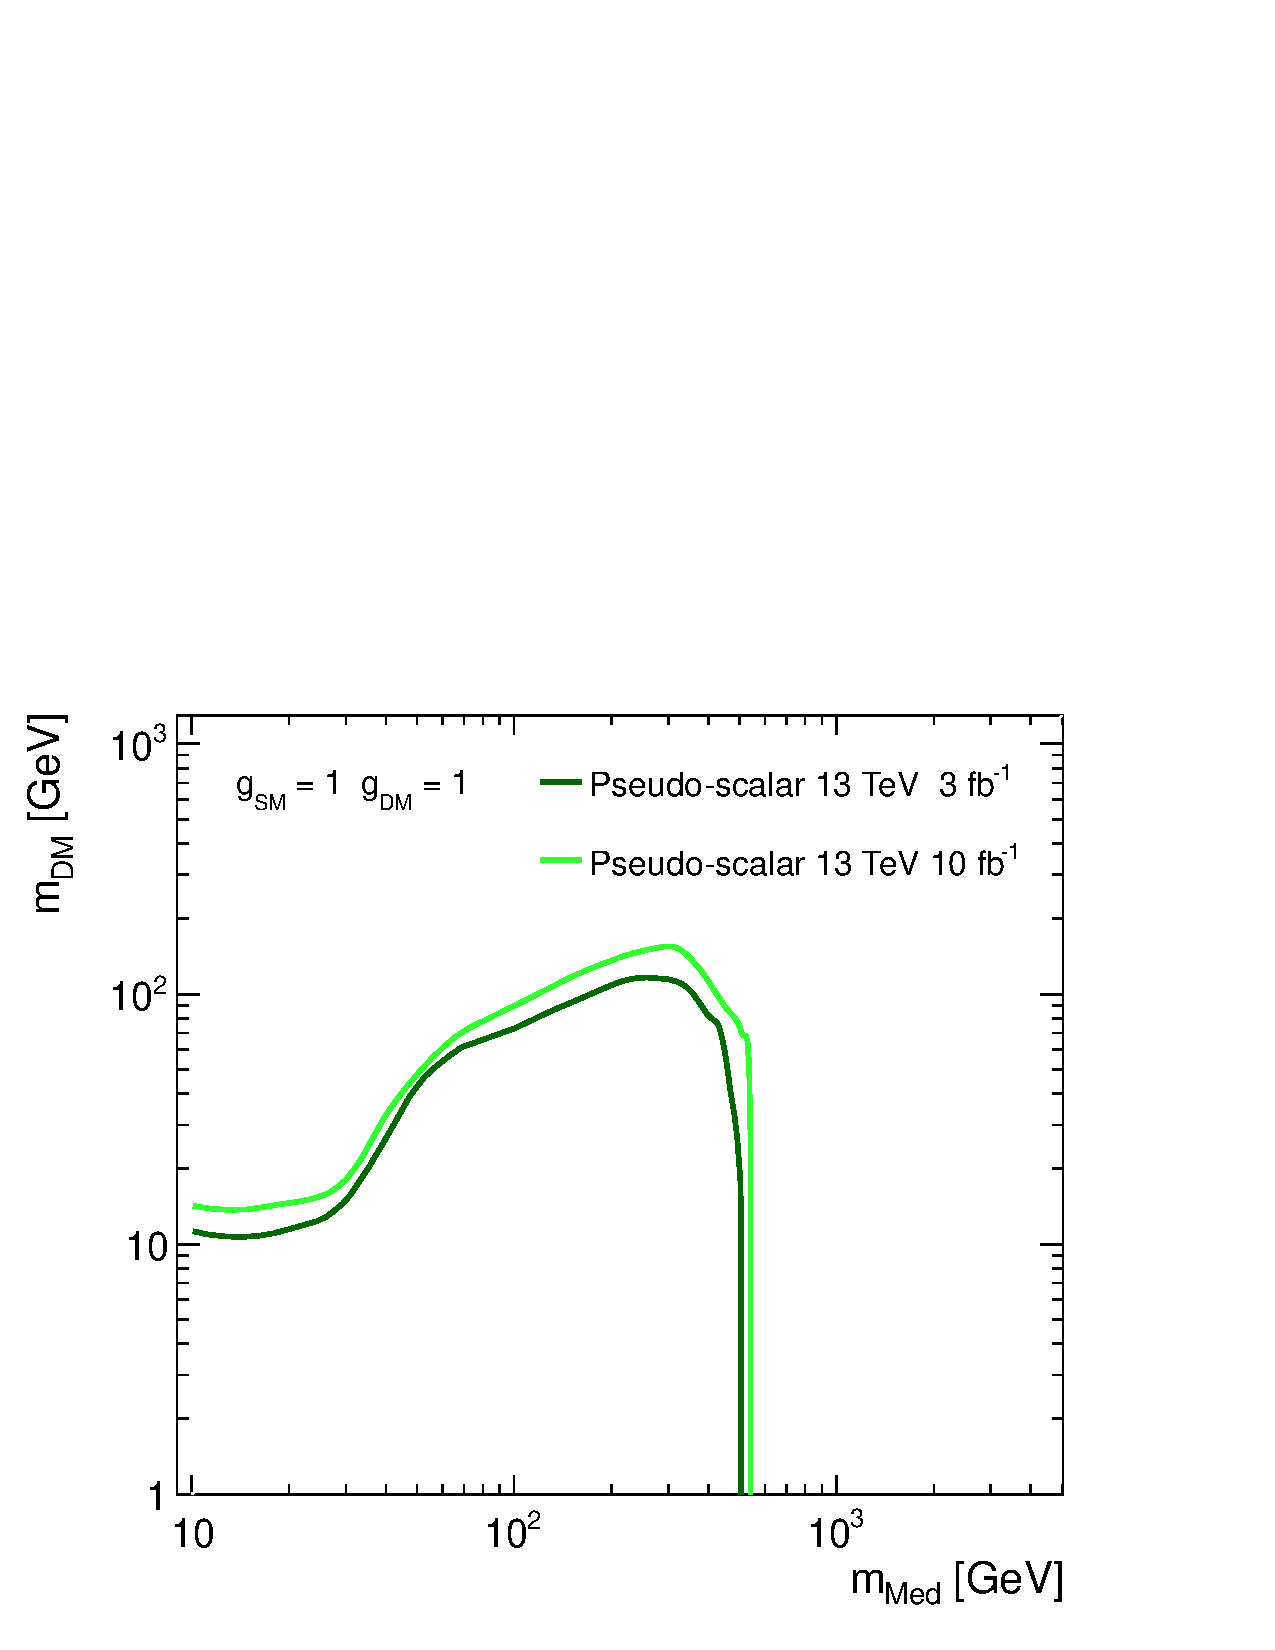
\includegraphics[width=0.5\textwidth]{figures/DMplots/justPlog.pdf}}
  \caption{\label{fig:limits_P} Expected exclusion contours at 95\% CL for 3\fbinv and 10\fbinv using pseudo-scalar couplings. }
\end{figure}


\clearpage
\subsubsection{Heavy quark simplified models}

Following the concept of Minimal Flavor Violating (MFV) top and bottom quarks can play important roles in the phenomenology of dark matter events.
Scalar and pseudoscalar mediator models predict not only the monojet process described in Sec.~\ref{sec:dm_pscalar} but also production of dark matter in association
with top (or bottom) pairs. This results in signature with relative large jet multiplicities, in particular for DM$+t\bar{t}$ production and heavy jets. Our $\alpa_{\textrm{T}}$ is particular well designed for this signature and the aforementioned improvements for monojet-like and compressed events further improves the sensitivity. The events are produced in the same parameters space as detailed in Tab.~\ref{tab:DMgrid} using \textsc{MadGraph5\_aMC@NLO} 2.2.2 and using \textsc{Pythia 8} for the parton shower. Figure~\ref{fig:feynman_hf} show Feynman diagrams for the pair production of dark matter particles in association with pairs of heavy quarks.


\begin{figure}[h!]
  \centering
  \subfigure{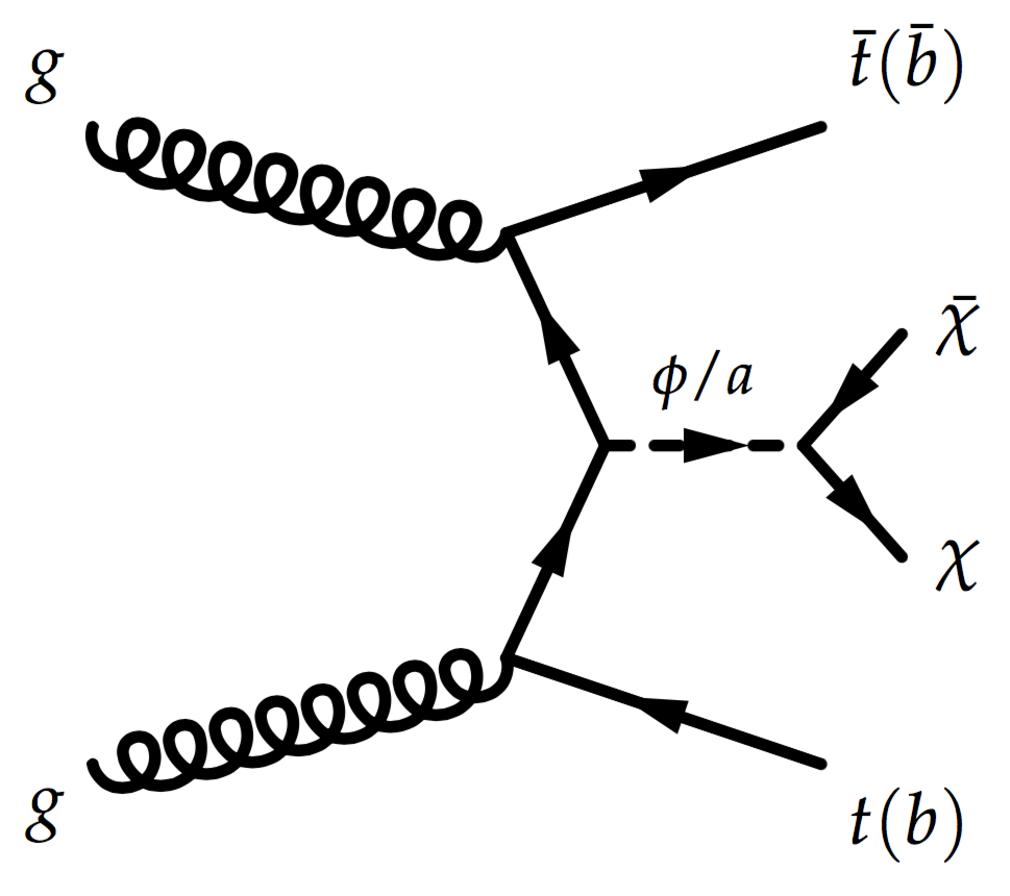
\includegraphics[width=0.5\textwidth]{figures/DMplots/feynman_hf.pdf}}
  \caption{Representative Feynman diagram showing the pair production of Dark Matter particles in association with $t\bar{t}$ or $b\bar{b}$̄). \cite{Abercrombie:2015wmb}}
  \label{fig:feynman_hf}
\end{figure}


Expected efficiencies and signal yields for nominal, asymmetric and total selection can be found for 3 fb$^{-1}$ in Table~\ref{tab:dmtt_S} and Table~\ref{tab:dmtt_P}.

\begin{table}[h!]
\centering
\begin{tabular}{l|lllll}
\hline
sample             & $\sigma$ [pb] & Sum Evts       & Evts Sym. Bin & Evts Asym. Bin & Eff  [\%]   \\\hline
Mchi1000\_MPhi1000 & 9.44E-09 & 0      & 0      & 0     & 21.45 \\
Mchi1000\_MPhi5000 & 1.71E-09 & 0      & 0      & 0     & 22.38 \\
Mchi100\_MPhi100   & 3.24E-04 & 0.13   & 0.1    & 0.03  & 13.86 \\
Mchi100\_MPhi195   & 1.07E-03 & 0.38   & 0.28   & 0.11  & 11.91 \\
Mchi100\_MPhi500   & 4.59E-03 & 2.12   & 1.6    & 0.53  & 15.41 \\
Mchi10\_MPhi10     & 9.47E-02 & 4.57   & 2.97   & 1.61  & 1.61  \\
Mchi10\_MPhi200    & 9.32E-02 & 26.39  & 19.09  & 7.3   & 9.44  \\
Mchi10\_MPhi5000   & 6.11E-08 & 0      & 0      & 0     & 16.93 \\
Mchi150\_MPhi10    & 8.66E-05 & 0.04   & 0.03   & 0.01  & 15.44 \\
Mchi150\_MPhi295   & 3.96E-04 & 0.17   & 0.13   & 0.05  & 14.59 \\
Mchi150\_MPhi500   & 3.77E-03 & 1.73   & 1.3    & 0.44  & 15.33 \\
Mchi1\_MPhi100     & 6.72E-01 & 75.76  & 51.18  & 24.58 & 3.76  \\
Mchi1\_MPhi2000    & 1.03E-05 & 0.01   & 0.01   & 0     & 19.47 \\
Mchi1\_MPhi20      & 1.04E+01 & 184.68 & 111.12 & 73.56 & 0.59  \\
Mchi1\_MPhi5000    & 6.15E-08 & 0      & 0      & 0     & 16.78 \\
Mchi1\_MPhi50      & 2.94E+00 & 132.23 & 76.25  & 55.98 & 1.5   \\
Mchi500\_MPhi2000  & 5.78E-06 & 0      & 0      & 0     & 20.84 \\
Mchi500\_MPhi500   & 9.93E-07 & 0      & 0      & 0     & 18.86 \\
Mchi50\_MPhi10     & 1.91E-03 & 0.49   & 0.34   & 0.14  & 8.45  \\
Mchi50\_MPhi300    & 2.91E-02 & 11.67  & 8.42   & 3.24  & 13.38 \\
Mchi50\_MPhi50     & 2.33E-03 & 0.55   & 0.4    & 0.15  & 7.9  
\hline
\end{tabular}
\caption{Selected DM+$t\bar{t}$ scalar samples. Given are production cross section, event yields for 3 fb$^{-1 }$ for the various selections and the overall selection efficiency for $g_\textrm{DM}=g_\textrm{SM}=1$ \label{tab:dmtt_S}}
\end{tabular}
%\end{table}

\begin{table}[h!]
\centering
\begin{tabular}{l|lllll}
\hline
sample             & $\sigma$ [pb] & Sum Evts       & Evts Sym. Bin & Evts Asym. Bin & Eff  [\%]   \\\hline
Mchi1000\_MPhi1000 & 3.93E-08 & 0     & 0     & 0     & 20.87 \\
Mchi1000\_MPhi1995 & 1.10E-06 & 0     & 0     & 0     & 21.28 \\
Mchi100\_MPhi1000  & 3.84E-04 & 0.21  & 0.17  & 0.04  & 18.03 \\
Mchi100\_MPhi10    & 6.53E-04 & 0.26  & 0.19  & 0.08  & 13.43 \\
Mchi100\_MPhi300   & 4.01E-02 & 14.87 & 10.7  & 4.17  & 12.38 \\
Mchi10\_MPhi100    & 1.90E-01 & 50.82 & 35.61 & 15.21 & 8.91  \\
Mchi10\_MPhi15     & 1.85E-02 & 3.89  & 2.62  & 1.27  & 6.99  \\
Mchi10\_MPhi250    & 5.76E-02 & 20.79 & 14.76 & 6.03  & 12.03 \\
Mchi10\_MPhi50     & 3.01E-01 & 62.23 & 41.04 & 21.2  & 6.88  \\
Mchi150\_MPhi200   & 4.14E-04 & 0.18  & 0.13  & 0.05  & 14.18 \\
Mchi150\_MPhi5000  & 5.72E-08 & 0     & 0     & 0     & 18.05 \\
Mchi1\_MPhi1000    & 3.97E-04 & 0.21  & 0.17  & 0.04  & 17.97 \\
Mchi1\_MPhi10      & 4.38E-01 & 68.58 & 45.77 & 22.82 & 5.21  \\
Mchi1\_MPhi200     & 8.42E-02 & 27.67 & 19.6  & 8.07  & 10.95 \\
Mchi1\_MPhi300     & 4.01E-02 & 15.41 & 11.01 & 4.41  & 12.82 \\
Mchi50\_MPhi5000   & 6.87E-08 & 0     & 0     & 0     & 17.16 \\
Mchi50\_MPhi95     & 1.07E-02 & 3.01  & 2.08  & 0.93  & 9.36 \\
\hline
\end{tabular}
\caption{Selected DM+$t\bar{t}$ pseudo-scalar samples. Given are production cross section, event yields for 3 fb$^{-1 }$ for the various selections and the overall selection efficiency for $g_\textrm{DM}=g_\textrm{SM}=1$ \label{tab:dmtt_P}}
\end{tabular}
\end{table}



\clearpage
\subsubsection{Projected sensitivities}

Expected R values for simplified dark matter models using scalar and pseudo-scalar couplings are calculated for 3 fb$^{-1 }$ and 10 fb$^{-1 }$. Table~\ref{tab:dmtt_S_R_values} lists these
values for the DM and mediator masses $m_\textrm{DM}$, $m_\Phi$ recommended by the DM forum for the scalar operator. The corresponding results for the pseudo-scalar couplings are given in Table~\ref{tab:dmtt_P_R_values}. 

\begin{table}
  \centering
  \begin{tabular}{llll}
    \hline                      
    $m_\textrm{DM}$ & $m_\Phi$  & R 3 fb$^{-1}$ & R 10 fb$^{-1}$ \\ \hlin
    1       & 10      & 0.32    & 0.18 \\ \hline
    1       & 20      & 0.49    & 0.25 \\ \hline
    1       & 50      & 0.87    & 0.48 \\ \hline
    1       & 100     & 1.63    & 0.89 \\ \hline
    1       & 200     & 4.61    & 2.51 \\ \hline
    1       & 300     & 8.22    & 4.55 \\ \hline
    1       & 500     & 32.38   & 17.81 \\ \hline
    1       & 1000    & 277.75  & 148.25 \\ \hline
    10      & 10      & 24.31   & 13.56 \\ \hline
    10      & 15      & 17.81   & 9.53 \\ \hline
    10      & 50      & 1.02    & 0.57 \\ \hline
    10      & 100     & 1.73    & 0.94 \\ \hline
    10      & 200     & 4.14    & 2.32 \\ \hline
    10      & 250     & 6.34    & 3.55 \\ \hline
    50      & 10      & 224.50  & 124.25 \\ \hline
    50      & 50      & 191.63  & 104.25 \\ \hline
    50      & 95      & 99.25   & 54.00 \\ \hline
    50      & 200     & 5.83    & 3.30 \\ \hline
    50      & 300     & 8.22    & 4.52 \\ \hline
    100     & 10      & 776.75  & 412.75 \\ \hline
    100     & 100     & 654.00  & 336.63 \\ \hline
    100     & 195     & 263.25  & 147.91 \\ \hline
    100     & 300     & 8.47    & 4.77 \\ \hline
    100     & 500     & 36.88   & 20.56 \\ \hline
    100     & 1000    & 288.88  & 157.25 \\ \hline 
    150     & 10      & -       & 1056.25 \\ \hline
    150     & 200     & 1494.25 & 823.50 \\ \hline
    150     & 295     & 482.25  & 263.63 \\ \hline
    150     & 500     & 46.88   & 26.63 \\ \hline
    500     & 995     & -       4000.00 \\ \hline
    1000    & 10      & -       4000.00 \\ \hline
  \end{tabular}
  \caption{Projected R values for 3 fb$^{-1}$ and 10 fb$^{-1}$ for the scalar  DM+$t\bar{t}$ models.
    \label{tab:dmtt_S_R_values}}
\end{table}

\begin{table}[h!]
  \centering
  \begin{tabular}{llll}
    \hline                      
    $m_\textrm{DM}$ & $m_\Phi$  & R 3 fb$^{-1}$ & R 10 fb$^{-1}$ \\ \hline
    1       & 10      & 1.8     & 1.0 \\ \hline
    1       & 20      & 1.8     & 1.0 \\ \hline
    1       & 100     & 2.5     & 1.4 \\ \hline
    1       & 200     & 3.9     & 2.1 \\ \hline
    1       & 300     & 6.5     & 3.7 \\ \hline
    1       & 1000    & 250.3   & 136.6 \\ \hline
    10      & 10      & 35.1    & 19.2 \\ \hline
    10      & 15      & 29.1    & 16.1 \\ \hline
    10      & 50      & 2.0     & 1.1 \\ \hline
    10      & 100     & 2.4     & 1.3 \\ \hline
    10      & 200     & 3.8     & 2.1 \\ \hline
    10      & 250     & 5.0     & 2.8 \\ \hline
    50      & 50      & 107.3   & 59.3 \\ \hline
    50      & 95      & 37.4    & 21.0 \\ \hline
    50      & 5000    & -       & 4000.0 \\ \hline
    100     & 10      & 356.9   & 197.6 \\ \hline
    100     & 100     & 285.9   & 160.6 \\ \hline
    100     & 195     & 49.6    & 27.1 \\ \hline
    100     & 300     & 6.3     & 3.5 \\ \hline
    100     & 500     & 36.8    & 20.8 \\ \hline
    100     & 1000    & 269.3   & 145.9 \\ \hline
    150     & 10      & 851.8   & 427.0 \\ \hline
    150     & 200     & 509.3   & 282.3 \\ \hline
    150     & 295     & 72.6    & 40.9 \\ \hline
    150     & 500     & 35.1    & 19.4 \\ \hline
  \end{tabular}
  \caption{Projected R values for 3 fb$^{-1}$ and 10 fb$^{-1}$ for the pseudo-scalar DM+$t\bar{t}$ models.
    \label{tab:dmtt_P_R_values}}
\end{table}


\clearpage

\subsection{Effective Field Theory Models}


In particular during Run I of the LHC the use of effective field theory (EFT) has been used to relate various experimental signatures in a relatively model-independent way. 
The EFT approach is based on the assumption that new particles mediate the interactions between dark matter and standard model particles, but that these mediators are too heavy to be
 produced directly in experiments. Hence, the interactions can be described by a contact operator For each operator and dark matter mass $m_\textrm{DM}$ the relic abundance, direct detection signal
 and collider predictions depend on a single parameter $M^*$, which parameterises the coupling strength of the contact interaction. 

While this assumption can lead to stringent validity constraints we still provide a few samples that allow detailed benchmarks and comparisons between experiments and analyses approaches.
EFT models also for light and heavy quark final states have been analysed.
Table~\ref{tab:datasets_dm} lists the light jet EFT samples generated using full simulation for the Phys14 exercise. The samples are generated using a mediator mass $M=40$~TeV.

\begin{sidewaystable}[h!]
    \centering
    \caption{EFT dark matter samples for axial-vector and axial couplings using a mediator mass $M=40$~TeV \label{tab:datasets_dm}}
    \begin{tabular}{lr}
      \hline\hline
      \multicolumn{1}{c}{Data set}&\multicolumn{1}{c}{\# events}\tabularnewline
      \hline
      {\footnotesize \verb!/DarkMatter_Monojet_M-1_V_Tune4C_13TeV-madgraph/Phys14DR-PU20bx25_PHYS14_25_V1-v1/MINIAODSIM!   } &$197200$\tabularnewline
      {\footnotesize \verb!/DarkMatter_Monojet_M-100_V_Tune4C_13TeV-madgraph/Phys14DR-PU20bx25_PHYS14_25_V1-v1/MINIAODSIM! } &$189400$\tabularnewline
      {\footnotesize \verb!/DarkMatter_Monojet_M-1000_V_Tune4C_13TeV-madgraph/Phys14DR-PU20bx25_PHYS14_25_V1-v1/MINIAODSIM!} &$197200$\tabularnewline
      {\footnotesize \verb!/DarkMatter_Monojet_M-10_V_Tune4C_13TeV-madgraph/Phys14DR-PU20bx25_PHYS14_25_V1-v1/MINIAODSIM!  } &$191800$\tabularnewline
      {\footnotesize \verb!/DarkMatter_Monojet_M-1_AV_Tune4C_13TeV-madgraph/Phys14DR-PU20bx25_PHYS14_25_V1-v1/MINIAODSIM!  } &$191200$\tabularnewline
      {\footnotesize \verb!/DarkMatter_Monojet_M-10_AV_Tune4C_13TeV-madgraph/Phys14DR-PU20bx25_PHYS14_25_V1-v1/MINIAODSIM! } &$191200$\tabularnewline
      {\footnotesize \verb!/DarkMatter_Monojet_M-100_AV_Tune4C_13TeV-madgraph/Phys14DR-PU20bx25_PHYS14_25_V1-v1/MINIAODSIM!} &$191200$\tabularnewline
\hline
\end{tabular}
\end{sidewaystable}


Expected yields for total, nominal and asymmetric selections and efficiency for the axial-vector and vector EFT operators are shown in Table~\ref{tab:dm_mj_eft_yields}.
The projections correspond again to 3\fbinv.

\begin{table}[h!]
\centering
\begin{tabular}{llllll}
\hline
sample             & $\sigma$ [pb] & Sum Evts       & Evts Sym. Bin & Evts Asym. Bin & Eff  [\%]   \\\hline
\multicolumn{6}{c}{axial-vector}        \\\line
1    & 9.57E-01 & 554.17 & 329.48 & 224.68 & 19.3  \\
10   & 9.54E-01 & 554.94 & 332.06 & 222.88 & 19.39 \\
100  & 8.01E-01 & 507.55 & 305.86 & 201.68 & 21.12 \\
1000 & 4.66E-02 & 39.05  & 24.21  & 14.84  & 27.91 \\
\multicolumn{6}{c}{vector}        \\\line
110    & 9.55E-01 & 553.96 & 331.02 & 222.94 & 19.34 \\
100   & 9.05E-01 & 544.63 & 323.4  & 221.22 & 20.07 \\
1000  & 1.24E-01 & 102.45 & 63.73  & 38.72  & 27.46 \\
\hline
\end{tabular}
\caption{Yields for the light jet EFT samples for 3\fbinv.} 
\label{tab:dm_mj_eft_yields}
\end{table}



Table~\ref{tab:dm_mj_eft_rvalues} shows the R values obtained for 3\fbinv and 10\fbinv. The corresponding exclusion obtained for the reduced mass $M^*$ are displayed in Fig.~\ref{fig:MJ_EFT_limit}

\begin{table}[h!]
\centering
\begin{tabular}{lll}\hline
$m_{\textrm{DM}}$& 3\fbinv  & 10\fbinv \\\hline
5\multicolumn{3}{c}{axial-vector}        \\\line
1             & 0.41 & 0.24 \\
10            & 0.40 & 0.23 \\
100           & 0.42 & 0.25 \\
1000          & 4.02 & 2.26 \\\hline
\multicolumn{3}{c}{vector}        \\\line
10            & 0.41 & 0.24 \\
100           & 0.40 & 0.24 \\
1000          & 1.55 & 0.87\\
\hline
\end{tabular}
\caption{Expected R values for the (axial)-vector EFT model for 3\fbinv and 10\fbinv.} 
\label{tab:dm_mj_eft_rvalues}
\end{table}



\begin{figure}[h!]
  \centering
  \subfigure{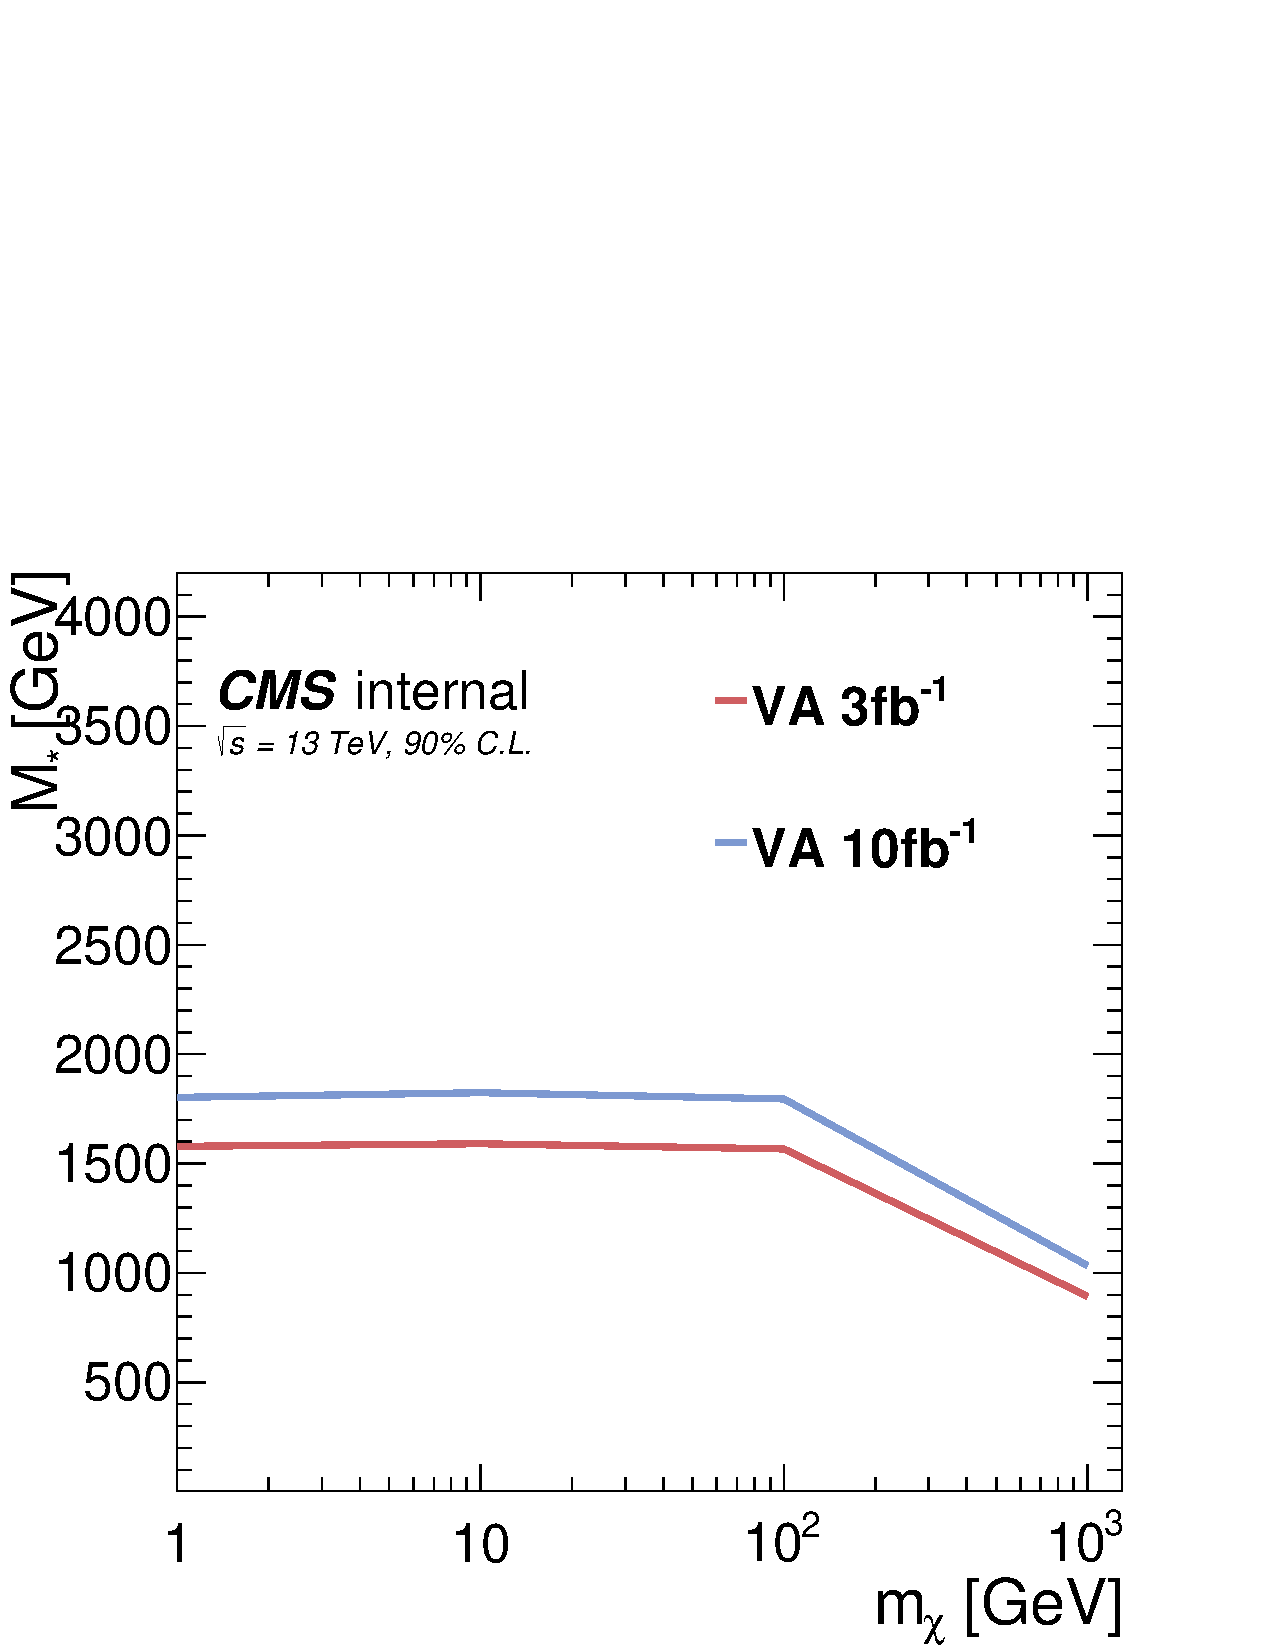
\includegraphics[width=0.5\textwidth]{figures/DMplots/limit_EFT_MJ_90.pdf}}
  \caption{\label{fig:MJ_EFT_limit} Expected limits on $M^*$at 90\% CL for 3\fbinv and 10\fbinv using the light jet axial-vector EFT models. }
\end{figure}



\clearpage


Table~\ref{tab:datasets_dmtt} lists the heavy uark jet EFT samples generated using full simulation for the Phys14 exercise. The samples are generated using a mediator mass $M=40$~TeV.

\begin{sidewaystable}[h!]
    \centering
    \caption{EFT dark matter samples for scalar DM+$t\bar{t}$ samples using a mediator mass $M=1x$~TeV. The cross sections are scaled by $10^6$ which corresponds to $M_*=100$ GeV \label{tab:datasets_dmtt}}
    \begin{tabular}{lr}
      \hline\hline
      \multicolumn{1}{c}{Data set}&\multicolumn{1}{c}{\# events}\tabularnewline
      \hline
      {\footnotesize \verb!/TTDMDMJets_M1GeV_Tune4C_13TeV-madgraph-tauola/Phys14DR- PU20bx25_PHYS14_25_V1-v1/MINIAODSIM!}   & 1.32 \tabularnewline
      {\footnotesize \verb!/TTDMDMJets_M10GeV_Tune4C_13TeV-madgraph-tauola/Phys14DR- PU20bx25_PHYS14_25_V1-v1/MINIAODSIM!}  & 1.32 \tabularnewline
      {\footnotesize \verb!/TTDMDMJets_M50GeV_Tune4C_13TeV-madgraph-tauola/Phys14DR- PU20bx25_PHYS14_25_V1-v1/MINIAODSIM!}  & 1.19 \tabularnewline
      {\footnotesize \verb!/TTDMDMJets_M200GeV_Tune4C_13TeV-madgraph-tauola/Phys14DR- PU20bx25_PHYS14_25_V1-v1/MINIAODSIM!} & 0.63 \tabularnewline
      {\footnotesize \verb!/TTDMDMJets_M600GeV_Tune4C_13TeV-madgraph-tauola/Phys14DR- PU20bx25_PHYS14_25_V1-v1/MINIAODSIM!} & 0.10 \tabularnewline
      {\footnotesize \verb!/TTDMDMJets_M1000GeV_Tune4C_13TeV-madgraph-tauola/Phys14DR- PU20bx25_PHYS14_25_V1-v1/MINIAODSIM!}& 0.02 \tabularnewline
      \hline \hline
\end{tabular}
\end{sidewaystable}

Expected yields for total, nominal and asymmetric selections and efficiency for the axial-vector and vector operators are shown in Table~\ref{tab:dm_dmtt_EFT_g1}.
The projections correspond again to 3\fbinv

\begin{table}[h!]
\centering
\begin{tabular}{llllll}
\hline
sample             & $\sigma$ [pb] & Sum Evts       & Evts Sym. Bin & Evts Asym. Bin & Eff  [\%]   \\\hline
1    & 1.32E+00 & 645.69 & 470.29 & 175.4  & 16.31 \\
10   & 1.32E+00 & 650.53 & 476.32 & 174.21 & 16.4  \\
50   & 1.19E+00 & 636.05 & 463.57 & 172.48 & 17.86 \\
200  & 6.30E-01 & 375.29 & 282.03 & 93.26  & 19.85 \\
600  & 1.04E-01 & 69.36  & 55.21  & 14.15  & 22.27\\
1000 & 1.58E-02 & 11.1   & 9.15   & 1.95   & 23.34 \\
\hline
\end{tabular}
\caption{Production cross section, event yields scaled to 3 fb$^{-1 }$ for the various selections and the overall selection efficiency for DM+$t\bar{t}$ EFT samples}
\label{tab:dm_dmtt_EFT_g1}
\end{table}


Table~\ref{tab:dm_dmtt_eft_rvalues} shows the R values obtained for 3\fbinv and 10\fbinv. The corresponding exclusion on the reduced mass $M^*$ are shown in Fig.~\ref{fig:DMtt_EFT_limit}


\begin{table}[h!]
\centering
\begin{tabular}{lll}\hline
$m_{\textrm{DM}}$& 3\fbinv  & 10\fbinv \\\hline
1            & 0.13 & 0.07 \\
10           & 0.09 & 0.05 \\
50           & 0.09 & 0.05 \\
200          & 0.13 & 0.07 \\
600          & 0.53 & 0.28 \\
1000         & 2.63 & 1.36 \\
\hline
\end{tabular}
\caption{Expected R values for the DM+$t\bar{t}$ EFT model for 3\fbinv and 10\fbinv. \label{tab:dm_dmtt_eft_rvalues}} 
\end{table}


\begin{figure}[h!]
  \centering
  \subfigure{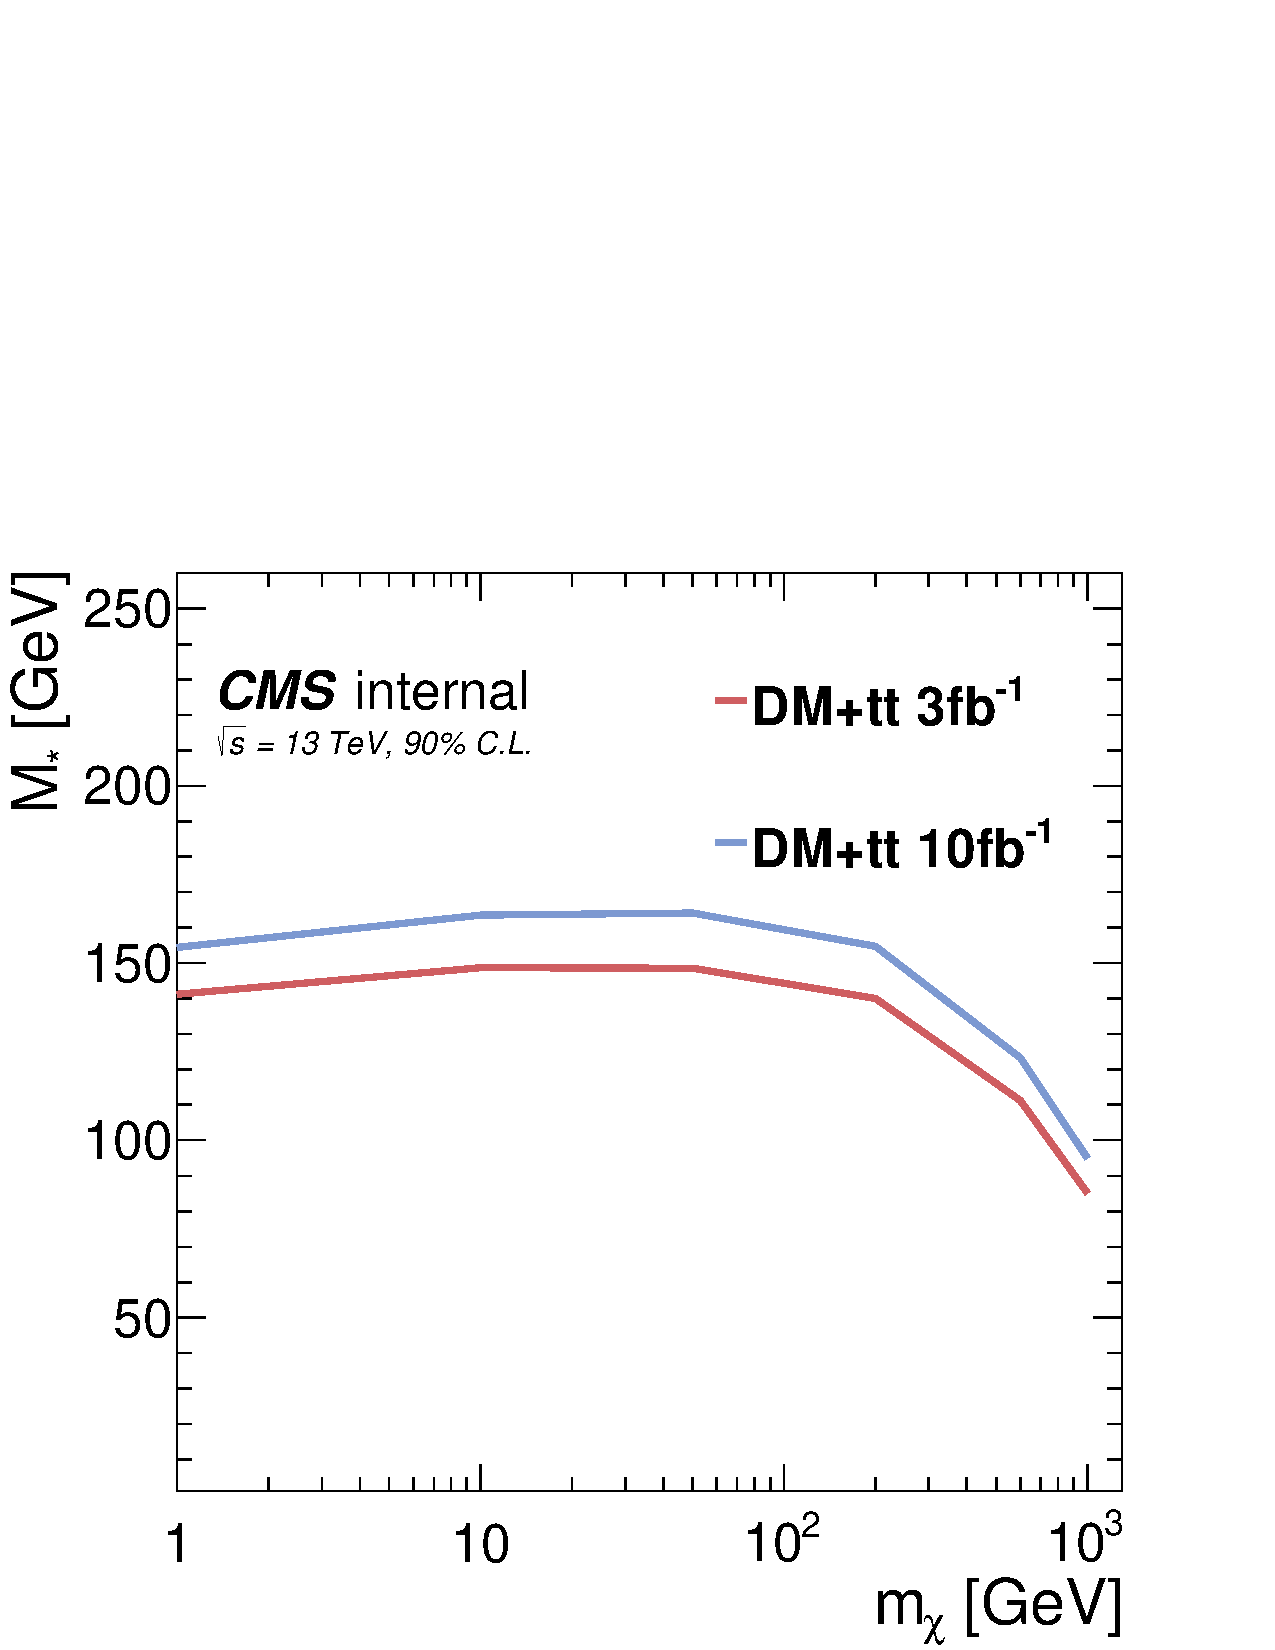
\includegraphics[width=0.5\textwidth]{figures/DMplots/limit_DMtt_EFT_90.pdf}}
  \caption{\label{fig:DMtt_EFT_limit} Expected limits on $M^*$at 90\% CL for 3\fbinv and 10\fbinv using a scalar DM+$t\bar{t}$ EFT model. }
\end{figure}



\clearpage
\subsection{Sensitivity considerations}

The RA1 analysis considers a variety of possible signal regions and combines the ten most sensitive bins for the final results. For each signal model and parameter space mass points we retain the information of the most sensitive bins as determined by the analysis. We present for points approximately at the largest $m_\textrm{DM}$, $m_\phi$ exclusion expected for 3\fbinv for the main models analyzed.

Tables~\ref{tab:bestBins_V_3fb}-\ref{tab:bestBins_P_3fb} list the five most sensitive bins for light jet axial, vector-axial, scalar and pseudo-scalar models. Tables~\ref{tab:bestBins_tt_P_3fb}, ~\ref{tab:bestBins_tt_P_3fb} shows the corresponding values for the scalar and pseud-scalar DM+$t\bar{t}$ models. Each table lists the most sensitive category in terms of jet multiplicity, nominal or asymetric selection (the latter denoted by 'a' added to the jet multiplicity bin), \HT~and \MHT~ bin.


\begin{table}[h!]
  \centering
  \begin{tabular}{lllll}
    \hline
    \textbf{A mDM150 mPhi1000 mht} & bgTtw & bgZinv & Signal & Significance \\ \hline
    htBin 600-800 cat eq2a eq0b mht 650 & 1.43 & 4.70 & 4.04 &1.26 \\
    htBin 800-Inf cat eq2j eq0b mht 850 & 1.83 & 9.82 & 5.45 &1.09 \\
    htBin 800-Inf cat eq3j eq0b mht 850 & 1.80 & 9.01 & 4.58 &0.91 \\
    htBin 600-800 cat eq2j eq0b mht 675 & 2.26 & 8.71 & 4.33 &0.86 \\
    htBin 800-Inf cat eq3a eq0b mht 725 & 1.79 & 6.91 & 2.87 &0.58 \\
    \hline
  \end{tabular}
  \caption{Five most sensitive bins in the light jet axial-vector model for $m_\textrm{DM}$=150 GeV and $m_\phi$=1000 GeV and 3\fbinv. \label{tab:bestBins_A_3fb}}
\end {table}


\begin{table}[h!]
  \centering
  \begin{tabular}{lllll}
    \hline
    \textbf{V mDM500 mPhi995 mht} & bgTtw & bgZinv & Signal & Significance \\ \hline
    htBin 800-Inf cat eq3j eq0b mht 850 & 1.80 & 9.01 & 1.31 &0.26 \\
    htBin 600-800 cat eq3j eq0b mht 650 & 2.23 & 8.27 & 0.63 &0.11 \\
    htBin 600-800 cat eq2j eq0b mht 625 & 2.67 & 8.86 & 0.51 &0.10 \\
    htBin 600-800 cat eq4j eq0b mht 575 & 2.97 & 9.53 & 0.51 &0.10 \\
    htBin 400-600 cat eq4j eq0b mht 475 & 3.09 & 8.51 & 0.45 &0.08 \\
    \hline
  \end{tabular}
  \caption{Five most sensitive bins in the light jet vector model for $m_\textrm{DM}$=500 GeV and $m_\phi$=995 GeV and 3\fbinv. \label{tab:bestBins_V_3fb}}
\end {table}


\begin{table}[h!]
  \centering
  \begin{tabular}{lllll}
    \hline
    \textbf{S mDM10 mPhi50 mht} & bgTtw & bgZinv & Signal & Significance \\ \hline
    htBin 600-Inf cat ge5a eq0b mht 425 & 0.74 & 2.04 & 2.59 &1.17 \\
    htBin 400-600 cat eq3a eq1b mht 300 & 2.37 & 2.24 & 2.59 &0.91 \\
    htBin 800-Inf cat eq2j eq0b mht 550 & 2.20 & 6.22 & 2.59 &0.67 \\
    htBin 800-Inf cat eq3j eq0b mht 550 & 2.86 & 7.77 & 2.59 &0.52 \\
    htBin 350-400 cat eq3j eq1b mht 250 & 24.57 & 13.34 & 5.18 &0.39 \\
    \hline
  \end{tabular}
  \caption{Five most sensitive bins in the light jet vector model for $m_\textrm{DM}$=10 GeV and $m_\phi$=50 GeV and 3\fbinv. \label{tab:bestBins_S_3fb}}
\end {table}


\begin{table}[h!]
  \centering
  \begin{tabular}{lllll}
    \hline
    \textbf{P mDM1 mPhi20 mht} & bgTtw & bgZinv & Signal & Significance \\ \hline
    htBin 300-350 cat eq4j eq0b mht 250 & 6.97 & 10.18 & 19.32 &2.77 \\
    htBin 250-300 cat eq3a eq1b mht 275 & 4.47 & 6.15 & 9.66 &2.00 \\
    htBin 350-400 cat eq2j eq1b mht 275 & 4.35 & 7.52 & 9.66 &1.80 \\
    htBin 400-600 cat ge5a eq0b mht 275 & 16.25 & 15.00 & 19.32 &1.70 \\
    htBin 350-400 cat eq3j eq1b mht 150 & 30.64 & 12.73 & 19.32 &1.26 \\
    \hline
  \end{tabular}
  \caption{Five most sensitive bins in the light jet vector model for $m_\textrm{DM}$=1 GeV and $m_\phi$=20 GeV and 3\fbinv. \label{tab:bestBins_P_3fb}}
\end {table}



\begin{table}[h!]
  \centering
  \begin{tabular}{lllll}
    \hline
    \textbf{DMtt S Mchi10 MPhi50 g1 mht} & bgTtw & bgZinv & Signal & Significance \\ \hline
    htBin 800-Inf cat ge5j ge3b mht 300 & 2.04 & 0.21 & 0.88 &0.42 \\
    htBin 800-Inf cat ge5j eq2b mht 650 & 0.36 & 0.27 & 0.44 &0.28 \\
    htBin 600-800 cat ge5j eq2b mht 0 & 11.31 & 0.52 & 1.76 &0.23 \\
    htBin 400-600 cat eq4j ge3b mht 175 & 3.25 & 0.32 & 0.44 &0.19 \\
    htBin 400-600 cat ge5j eq1b mht 225 & 59.16 & 9.94 & 4.41 &0.17 \\
    \hline
  \end{tabular}
  \caption{Five most sensitive bins in the heavy jets scalar model for $m_\textrm{DM}$=10 GeV and $m_\phi$=50 GeV and 3\fbinv. \label{tab:bestBins_tt_S_3fb}}
\end {table}



\begin{table}[h!]
  \centering
  \begin{tabular}{lllll}
    \hline
    \textbf{DMtt P Mchi1 MPhi20 g1 mht} & bgTtw & bgZinv & Signal & Significance \\ \hline
    htBin 400-600 cat ge5j eq1b mht 375 & 3.04 & 1.67 & 0.30 &0.11 \\
    htBin 800-Inf cat ge5j eq1b mht 775 & 0.42 & 1.40 & 0.18 &0.11 \\
    htBin 800-Inf cat ge5j eq2b mht 175 & 18.63 & 1.55 & 0.90 &0.11 \\
    htBin 800-Inf cat ge5j eq2b mht 325 & 4.94 & 0.79 & 0.36 &0.09 \\
    htBin 400-600 cat ge5j eq1b mht 275 & 23.79 & 6.53 & 0.78 &0.06 \\
    \hline
  \end{tabular}
  \caption{Five most sensitive bins in the heavy jets pseudo-scalar model for $m_\textrm{DM}$=1 GeV and $m_\phi$=20 GeV and 3\fbinv. \label{tab:bestBins_tt_P_3fb}}
\end {table}



%%____________________________________________________________________________||
